%%
%%  Hochschule für Technik und Wirtschaft Berlin --  Abschlussarbeit
%%
%%  Hauptdokument
%%
%%%%%%%%%%%%%%%%%%%%%%%%%%%%%%%%%%%%%%%%%%%%%%%%%%%

%% Einstellungen und Anpassungen
\input{settings/settings}  		% Import der Pakete und Stil des Dokuments
\input{settings/adjustments} 	% Weitere Pakete und Anpassungen (Sprache, Quellenverwaltung, etc.)
\input{settings/titlepage}		% Layout der Titelseite

%%%%%%%%%%%%%%%%%%%%%%%%%%%%%%%%%%%%%%%%%%%%%
% Im folgenden Bereich müssen Sie Anpassungen für das Deckblatt der Arbeit vornehmen!
%%%%%%%%%%%%%%%%%%%%%%%%%%%%%%%%%%%%%%%%%%%%%
%
%% Titel und Author 
%\titel{Wasseroberflächenüberwachung des Nachklärbeckens XY [am Klärwerk Waßmannsdorf] durch Mikrocontroller-Aufbau mit Semantischer Segmentierung über ein Neuronales Netzwerk - Schlagwörter: embedded System, Sensorik und Aktorik, mechanische Reinigung, große Namen!. Größen: Kosten, Effizienz, Robustheit}
\titel{Entwicklung eines Edge-Computing-Systems zur autonomen Wasseroberflächendetektion mittels semantischer Segmentierung auf einem Single-Board Computer in einer Air-Gap-Umgebung}
%\titel{Echtzeit Wasseroberflächenüberwachung und -reinigung eines Nachklärbeckens durch eingebettetes Air Gap System mittels Semantischer Segmentierung und CNN}
\autor{Elias Albrecht}
\matrikelnr{s0589247}
%% Version und Abgabedatum
\version{0.2$\alpha$} 	%ToDo: wird derzeit noch nicht genutzt
\datum{07.09.2026}   	% Abgabedatum der Arbeit
%% Typ der Arbeit
\thesistyp{Bachelorarbeit}
%\thesistyp{Bachelorarbeit}
\abschluss{Bachelor of Engineering (B. Eng.)}
%\abschluss{Bachelor of Engineering (B. Eng.)}
%% Betreuer
\firstExaminer{Prof.~Dr.-Ing. Jochen Kerdels}
\secondExaminer{B. Eng. Christian Rank}
%% Fachbereich
\fachbereich{1 -- Energie und Information --}
\studiengang{Computer Engineering}
%%%%%%%%%%%%%%%%%%%%%%%%%%%%%%%%%%%%%%%%%%%%%
% Ende des Bereichs für Anpassungen
%%%%%%%%%%%%%%%%%%%%%%%%%%%%%%%%%%%%%%%%%%%%%
%% Metadaten zu PDF hinzufügen
\hypersetup{
pdftitle = {\thetitel},
pdfsubject = {\thethesistyp},
pdfauthor = {\theautor},
%pdfkeywords = {Stichwort1, Stichwort2 ...} ,
pdfcreator = {LaTeX with hyperref},
pdfproducer = {pdflatex}
}
%% Pfad zu den Bildern




%% Current Bug-Fixes
% 2024-02 
% Error-Message ! Argument of \MT@gobble@to@nil has an extra }.
% https://tex.stackexchange.com/questions/702778/argument-of-mtgobbletonil-has-an-extra
\microtypesetup{nopatch=item}

%% Custom includes go here!!!



%%%%%%%%%%%%%%%%%%%%%%%%%%%%%%%%%%%%%%%%%%%%%
%% Start des Dokuments
%%%%%%%%%%%%%%%%%%%%%%%%%%%%%%%%%%%%%%%%%%%%%
\begin{document}

%% Deckblatt erzeugen
\maketitle

%% Inhaltsverzeichnis erstellen
%\cleardoubleoddpage
\pagenumbering{Roman}
\tableofcontents \clearpage
%%%%%%%%%%%%%%%%%%%%%%%%%%%%%%%%%%%%%%%%%%%%%
%%%%%%%%%%%%%%%%%%%%%%%%%%%%%%%%%%%%%%%%%%%%%
%% In diesem Bereich müssen Sie Anpassungen für den Inhalt der Arbeit vornehmen!
%% Kurzzusammenfassung
% !TEX root = ../Thesis.tex
%%
%%  Hochschule für Technik und Wirtschaft Berlin --  Abschlussarbeit
%%
%%  Abstract - Deutsch
%%
%%%%%%%%%%%%%%%%%%%%%%%%%%%%%%%%%%%%%%%%%%%%%%%%%%%%


\section*{Kurzfassung}



%Motivation, Fragestellung, Methodik, Ergebnisse, Schlussfolgerungen

%\input{Abstract_en.tex}
\clearpage

%% Hauptteil
%\cleardoubleoddpage
\pagenumbering{arabic}



% !TEX root = ../Thesis.tex
%%
%%  Hochschule für Technik und Wirtschaft Berlin --  Abschlussarbeit
%%
%% Kapitel 1
%%
%%

\chapter{Einleitung} \label{Einleitung}

\section{Aufgabenbeschreibung} \label{Aufgabenbeschreibung}

Im Rahmen dieser Bachelorarbeit soll eine Lösung geschaffen werden, die eine Videoüberwachung von Wasserbecken ermöglicht. Das System hat den Anspruch robust gegenüber Witterungsbedingungen zu sein und muss den lokalen Gegebenheiten entsprechen. An das Projekt wird die Anforderung gestellt, die gesammelten Bilddaten weiterzugeben oder sich selbst der Verarbeitung anzunehmen.

Das bestehende System basiert auf einer timergesteuerten Reinigung des Wasserbeckens, was hinsichtlich des Verschmutzungsverhaltens unzureichend ist und sich ein Optimierungsbedarf in Bezug auf die Ablaufqualität, des Stromverbrauchs und der Reinigungsmenge abzeichnet. Messbare Anforderungen an die vorgebrachte Lösung bestehen in der Funktionalität einer Air-Gap-Lösung, der Erkennungsqualität, dem verbundenen Wartungsaufwand und der resultierenden Stromersparnis im gesamten Kreislauf.  

\textbf{Ergänzen}: kurze Motivation/Problemkontext (Schwimmschlamm, Einfluss auf Ablaufqualität/Betrieb), sowie klare Zielsetzung als messbare Anforderungen (z.B. Offline/Air-Gap, Latenz, Erkennungsqualität, Wartungsaufwand). Außerdem Beitrag/Abgrenzung: was ist neu gegenüber Timerbetrieb, klassischer Bildverarbeitung oder Sensorik?

In dem weiteren Verfahren werden die Daten zum Training von einem und zur Verarbeitung durch ein Neuronales Netzes eingesetzt. Anhand der Resultate soll die vorhandene Vorrichtung am Nachklärbecken anlaufen.

Mittels Recherche und Rücksprache soll eine Abwägung hinsichtlich der tauglichsten Lösung stattfinden. Der beschlossene Ansatz wird als Prototyp aufgebaut und hinsichtlich seiner Funktionalität bewertet und optimiert. Mit diesem Vorgehen wird angestrebt, am Ende der Arbeit einen gezielten Vergleich der Kosten- und Ressourcenersparnisse aufzuzeigen, was den Grundstein für eine eventuelle Fortsetzung des Projekts legen soll.


\section{Herangehensweise}


In Kapitel \ref{Grundlagen} werden im Rahmen dieser Arbeit relevante Bezeichnungen erläutert, die aus den Bereichen der Mathematik, Technik aber auch spezifisch aus dem Umfeld des Klärwerks stammen.
Insbesondere sicherheitsrelevante Standards und Verfahren werden dargelegt, um die Ausgangsposition zu beschreiben. Software und Hardware, die in Anbetracht der Problemstellung Anwendung finden können, werden vorgestellt und hinsichtlich ihrer Nützlichkeit analysiert. Insbesondere auch Umgebungen und Betriebssysteme werden überprüft und auf ihren Nutzen getestet. Die Wahl fiel auf Linux Mint, da es wie das Originale Raspberry Pi OS auf Debian basiert und sich damit wenige Komplikationen ergeben. Ähnliche Distributionen eignen sich ebenfalls und stellen eine Frage der persönlichen Preferenz dar. 

Anschließend wird sich mit der Analyse der unterschiedlichen Ansätze und Bewertung dieser befasst. Es werden im Vorhinein Parameter allgemein definiert, die die Ansprüche an das Projekt klären. Auf dieser Basis erfolgt eine unvoreingenommene Entscheidung, die zum Abschluss der Arbeit kritisch bewertet wird. 

Im Kapitel \ref{Implementierung} werden die einzelnen Aspekte der Implementierung wie die Vorbereitung des Rechners, das Konfigurieren des Raspberry PIs oder die Montage am Nachklärbecken beschrieben.  
 
Es wird daraufhin anhand der Testverfahren gezeigt, welche Wasser- und Stromersparnisse sich durch den bedarfsorientierten Betrieb ergeben und wie stabil das System ist. Diese Tests werden aufgestellt und genauer beschrieben.

Im letzten Kapitel \ref{Fazit} werden die Tests ausgewertet und die Erfüllung der Anforderungen überprüft. Die Anfangs- und Endzustand werden auf ihre Unterschiede hin analysiert und verglichen. Die Skalierbarkeit der Lösung wird betrachtet und eine Fazit des Arbeitsprozesses gezogen. 







% !TEX root = ../Thesis.tex
%%
%%  Hochschule für Technik und Wirtschaft Berlin --  Abschlussarbeit
%%
%% Kapitel 2 - Grundlagen
%%
%%


\chapter{Grundlagen} \label{Grundlagen}



\section{Begriffserklärungen}

Da \textbf{\textit{Klärwerke}} hinsichtlich ihrer Funktion in der Informatik grundsätzlich selten betrachtet werden, wird im folgenden die Quintessenz für die Betrachtung der Problemstellung aufgebaut. Hierbei geht es insbesondere um grundsätzliche Bestandteile, aber auch lokal spezifische Gegebenheiten, die technisch, chemisch und informationselektronisch dargelegt werden.

Die Grundlagen für Faltbare Neuronale Netzwerke (CNNs) werden erläutert, wobei auch auf die zugrunde liegende Mathematik eingegangen wird. Zusätzlich erfolgt eine tabellarische Aufführung der Datensätze, der Arten von Neuronalen Netzwerken und den Verfahren zur Segmentierung zur Übersichtlichkeit. 

Um die später vorgestellten Übertragungstechniken und Kommunikationstechnologien besser einordnen zu können, wird zu Beginn auf das OSI-Modell \index{OSI-Modell}eingegangen.

Außerdem werden weitere Begriffe erläutert, die helfen sollen, die zu implementierende Lösung einzugruppieren. Teilweise handelt es sich um englische Begriffe, weil diese auch in der deutschen Literatur gebräuchlicher sind.

\subsection{Klärwerk}

In Klärwerken wird das ankommende Abwasser in mehreren Schritten geklärt. Angefangen mit mechanischen Reinigungsprozessen wie dem Grobrechen, der größere Bestandteile aus dem Wasser herausfiltert, den Sand- und Fettfängen, deren Zweck die Nutzung von Sedimentationsverfahren zur physischen Trennung von Lipiden und lockeren Gesteinsmaterialien ist. Anschließend werden Belebungslinien eingesetzt, die das Bakterienwachstum fördern sollen, um die Verarbeitung des Klärwassers voranzutreiben. Hierfür durchläuft das kommunale Abwasser mehrere Phasen, in denen mittels aerober Mikroorganismen die organischen Verunreinigungen verstoffwechselt werden. \cite{Jenkins_2004} \\
Am Ende dieser biologischen Prozesse wird das Wasser in Nachklärbecken weitergeleitet, die dieses in 4 Zonen unterteilt: Klarwasser-, Trenn-, Speicher- und Räum-/Eindickzone. Mittels sogennanter Räumer wird das Wasser gleichmäßig verteilt und der gram-positive Schlamm am Beckengrund in der Eindickzone abgeführt. Darüber befinden sich Speicher- und Trennzone, in denen sich die Partikel absetzen oder wie im Fall der gram-negativen Fadenorganismen auf der Klarwasserzone anreichern, wo sie Klär-/Blähschlamm bilden. Diese Art Schlamm wird ebenfalls gereinigt, da das übermäßige Wachstum zu einer Verdickung der Schicht führt. Das kann bewirken, dass der Ablauf des Klarwassers verschmutzt wird, weil sich die Schichten vermischen. Hierdurch entstehen weitere Probleme in der Klärung des Wassers, da die Qualitätsansprüche für (beispielsweise) eine Flockungsfiltration nicht erfüllt werden. \\ \\

\index{SSR}: Schwimmende-Schwimmschlamm-Räumer werden eingesetzt um über eine oder mehrere Förderschnecken den Oberflächenbelag an einem Schwimmschlamm-Schlürftrichter zu konzentrieren. Der Inhalt wird abgefördert, um die Oberfläche sauber zu halten, damit der Anteil an entsprechenden Fadenbakterien wie Microthrix Parvicella nicht überhand nimmt und das Gleichgewicht des Beckens stört.
Die bisherige Steuerung funktioniert über einen Timer, der zwischen Winter- und Sommerbetrieb umgeschalten wird, um auf die Veränderungen des Bakterienwachstums und der damit einhergehenden Oberflächen-
beschaffenheit annäherungsweise einzugehen. Da die biologischen Begebenheiten hierbei deutlich komplexer als ein simpler Zeitintervall sind, ergibt sich ein Optimierungsgedanke. 

\subsection{Neuronale Netzwerke}
Bereits im Jahr 1842 wurden programmierbare Rechner mit der Fähigkeit zur (menschlichen) Intelligenz erdacht, obwohl sie als einfache Maschinen erst über ein Jahrhundert später ins Leben gerufen wurden. Entsprechend alt ist der Grundgedanke von Apparaturen, die in ihren Zügen menschliche Denkeigenschaften verkörpern.
\cite{goodfellow_2016} \\ \\
Inzwischen hat sich viel getan über die anfänglichen Entwicklungen mit cybernetics in den 1940-60er Jahre als Entwicklung von Theorien zu biologischem Lernen und ersten Implementierungen zum Training eines einzelnen Neuronen mit dem \say{perceptron}, über connectionism, der mittels back-propagation das Training eines neuronalen Netzwerks mit ein oder zwei hidden layers ermöglichte und der aktuellen deep learning Entwicklung, die sich seit 2006 fortsetzt. \cite{Kim_2016} \\ \\
Mathematisch betrachtet liegen hier drei unterschiedliche Modelle vor. Die Ursprünge liegen im maschinellen Lernen, was hier in seinen Grundzügen erklärt sei. Beginnend mit dem Lernalgorithmus, der Grundzüge des Trainings auf Basis der Daten beschreibt. Eine allgemeine Definition von Tom Mitchell lautet: \say{A computer program is said to learn from experience \textbf{E} with respect to some class of tasks \textbf{T} and performance measure \textbf{P}, if its performance at tasks in \textbf{T}, as measured by \textbf{P}, improves with experience \textbf{E}.} 
Der Ausgestaltung der jeweiligen Kategorien werden nur von der Fantasie Grenzen gesetzt,was sich in differenzierten Ansätzen widerspiegelt. 

\subsubsection{Deep Learning}
Künstliche Intelligenz und Neuronale Netze stellen seit einigen Jahren den Status Quo dar, weswegen diese Technologie jedem ein Begriff sein sollte. Dennoch sei die grundlegende Funktionsweise hier erklärt, um das Basiswissen zu vereinheitlichen: 

\subsubsection{Semantische Segmentierung}
Die Semantische Segmentierung ist ein Konzept der Computer Vision, bei dem das erfasste Bild in mehrere Labels unterteilt wird. Nebeneinander liegende Pixel werden anhand von Alleinstellungsmerkmalen zusammengefasst.  Dieses Verfahren unterscheidet sich durch die strikte Aufteilung in allgemeine Schichten, während einzelne Objekte im Gegensatz zur Instanzsegmentierung oder panoptischen Segmentierung keine Rolle spielen. \cite{goodfellow_2016}

\begin{figure}[h]
    \centering
    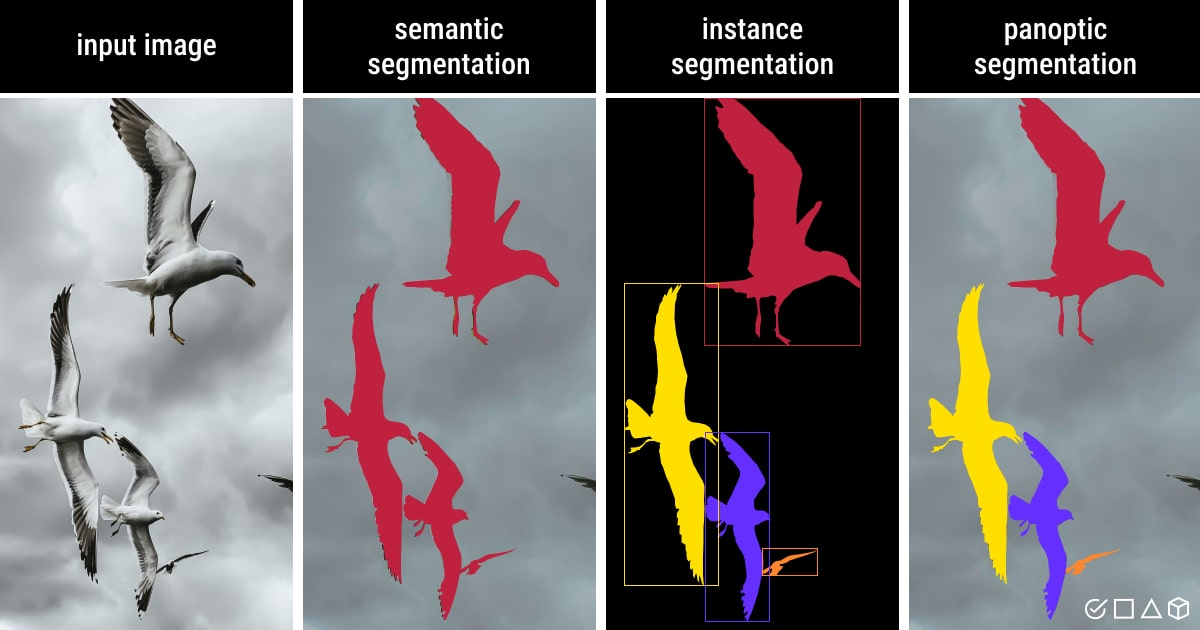
\includegraphics[width=0.8\linewidth]{pictures/segmentation_in_practice.jpg}
    \caption{Darstellung
    der Segmentierungsoptionen \cite{naminas_semantic_nodate} }
    \label{fig:Beispiel Segmentierung}
\end{figure}



\subsubsection{En- und Decoder}

En- und Decoder werden zur Verarbeitung sequentiellener Daten verwendet, bei denen es sich oft um sprachorientierte Modelle handelt. Hierbei werden Eingabesequenzen auf Ausgabesequenzen mit divergierender Länge übersetzt bzw. zugewiesen. In der Sprachübersetzung werden so anhand von trainierten Satzstrukturen Text aus dem Deutschen in das Englisch übersetzt, indem die Ausgabesequenz hinsichtlich ihrer Länge kontextuell modifizert wird.   

\begin{figure}[h]
    \centering
    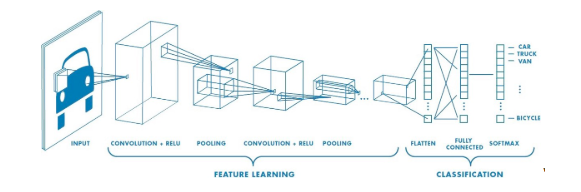
\includegraphics[width=0.8\linewidth]{pictures/De- und Encoder_hs_analysis.png}
    \caption{Darstellung der Verarbeitung von Encoder zu Decoder}
    \cite{}
    \label{fig:DeEncoder}
\end{figure}

Die Übersetzung erfolgt seitens des Encoders von dem ursprünglichen Datentyp hin zu einem vektoriellen und wird seitens des Decoders wieder zu zurückgewandelt. 
Sowohl De- als auch Encoder sind hierbei eigenständige Neuronale Netze, die in unterschiedlichen Varianten vorkommen können.
Die Basis eines Encoders ist ein zweischichtiges System, was sich einersauts aus einem Mechanismus zur Selbstüberwachung speist, der für die Gewichtung der Eingabe und damit der einzelnen Token und ihren Zusammenhang zuständig ist. 

\begin{equation}
    x_i = \sum_{j=1}^nw_{ji}x_{j}
\end{equation}

$x_j$ markiert hierbei einen eingegebenen Token (Wort) mit dem Index j in dem Eingabetext, während $x_i$ dem ausgegebenen Token mit dem Index i im Ausgabetext entspricht. Der Koeffizient $w_{ij}$ stellt die per Softmax-Funktion berechnete Gewichtung dar und damit die Wichtigkeit des Tokens für den Ausgabetext definiert. Manche Wortarten wie Verben haben zum Beispiel eine höhere Aussagekraft und dementsprechend Gewichtung als Füllwörter oder Artikel. Gleiches gilt in der Bildverarbeitung für die Kategorisierung einzelner Pixel in Hinblick auf ihre Klasse und der damit verbundenen Auswirkung auf Verarbeitung.  

Anschließend wird der entsprechende Token durch die Feed-Forward-Schicht eingebettet, was einer Positionskodierung in einem Satz anhand des Index (z.B. LLM) oder einer Einordnung in ein pixelweises, zweidimensionales Koordinatensystem entspricht (CNN, Bildverarbeitung). Aus beiden Schichten setzt sich der verborgene Zustand (Kontextvektor) zusammen, der als ein Element an den Decoder weitergegeben wird.

\begin{figure}[h]
    \centering
    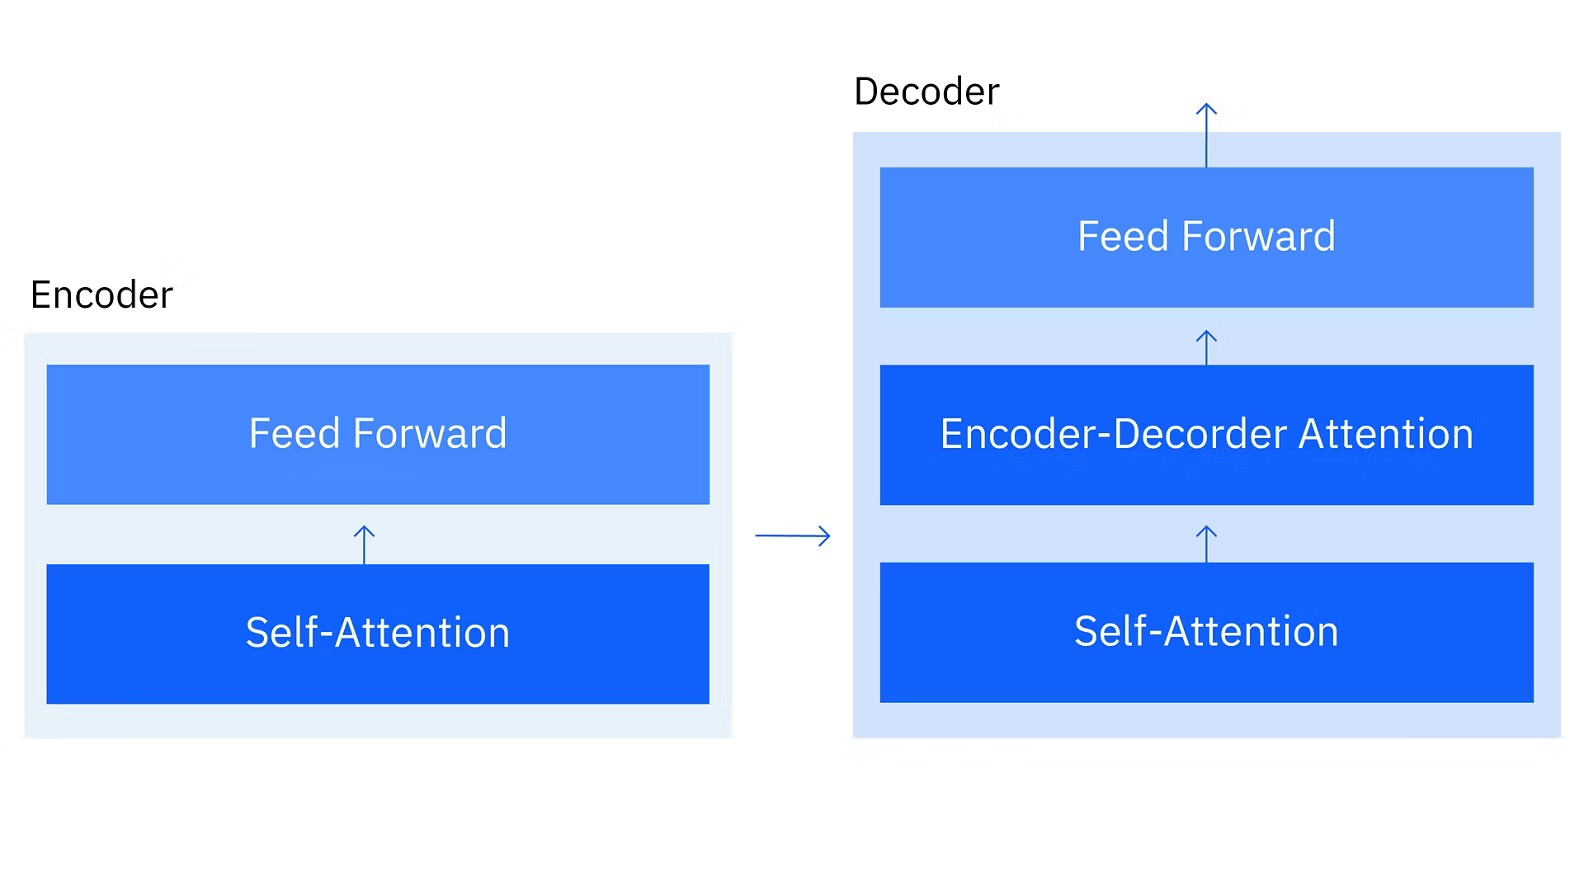
\includegraphics[width=0.8\linewidth]{pictures/encoder-decoder-image_ibm.png}
    \caption{Caption}
    \label{fig:Encoder-Decoder}
\end{figure}

Eine klassische Encoder-/Decoder-Architektur ist das U-Net. Dabei handelt es sich um eine Weiterentwicklung des FCNN mit dem Ziel, Bildsegmentierung mit kleinen Datensätzen und dennoch hoher Präzision zu verarbeiten. Wie der Name bereits andeutet, ist diese Architektur U-förmig aufgebaut: durch die hohe Anzahl an Kanälen, die Eigenschaften extrahieren, ist der kontrahierende Pfad ähnlicher Länge wie der expandierende. \cite{Ronneberger_2015} Dieses Verfahren wurde auch in diesem Projekt verwendet, um die Arbeit mit geringen Datenmengen zu vereinfachen und zugleich die Perfomanz hoch zu halten. Ein weiterer Vorteil besteht in der Nutzung von Skip-Connections, also dem partiellen Überspringen von Layern um qualitative Bilddetails zu erhalten.

\begin{figure}[h]
    \centering
    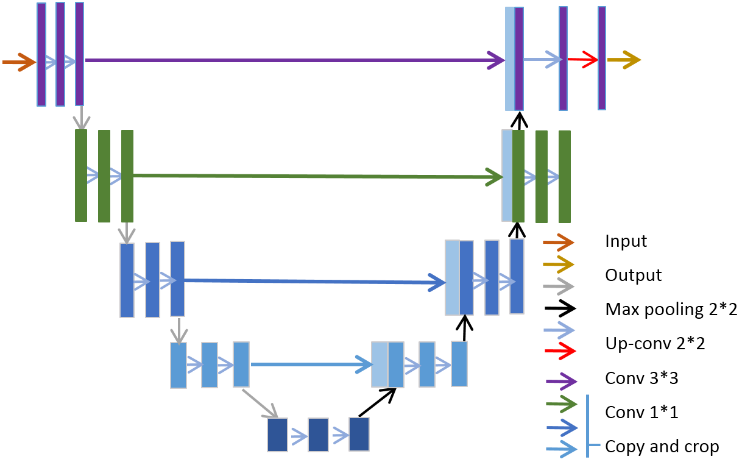
\includegraphics[width=0.5\linewidth]{pictures/The-architecture-of-Unet_researchgate.png}
    \caption{Caption}
    \label{fig:placeholder}
    \cite{Howard_2017}
\end{figure}


\textbf{Abschnitt schärfen:} U-Net als Encoder-Decoder-Architektur erklären (Skip-Connections, warum gut für Segmentierung) und passende Quelle(n) zitieren.

\subsubsection{Programme }

\subsection{Formeln}


Bayes Theorem
\begin{equation}
    Pr(H|E) = \frac{Pr(E|H)Pr(H)}{Pr(E|H)Pr(H) + Pr(E|!H)Pr(!H)}
\end{equation}

Das Bayes-Theorem dient der Berechnung der bedingten Wahrscheinlichkeit, dass A eintritt, wenn B bereits eingetreten ist, unter der Voraussetzung dass die Wahrscheinlichkeit von B unter der Bedingung von A vorliegt. 

Grundsätzlich ermöglicht dieser Satz also die Berechnung des Ereignisses $Pr(H|E)$ auf Grundlage von $Pr(E|H)$ mit dem Satz der totalen Wahrscheinlichkeit. 

Softmax-Funktion
\begin{equation}
    softmax(x)_i=\frac{e^{(x_i)}}{\Sigma_{j=1}^ne^{(x_j)}}
\end{equation}

Mittels der Softmax-Funktion wird ein Vektor als Input zu Wahrscheinlichkeiten überführt, deren Größe direkt damit korreliert. Ein hoher numerischer Wert geht mit einer entsprechenden Wahrscheinlichkeit einher. Mittels dieser Funktion wird dafür gesorgt, dass folgendes für die Summe der Ausgabewerte $S_a$ gilt: $S_a \leq 1$
Dieser Aspekt ist von hoher Relevanz für die Wahrscheinlichkeitsrechnung, in der nur dieses Spektrum für die Wahrscheinlichkeit von Interesse ist.

Schwellwertfunktion
\begin{equation}
     f(x)=\left\{\begin{array}{ll} 1, & x \geq a \\
         0, & sonst\end{array}\right. .
\end{equation}

Sigmoid-Funktion
\begin{equation}
     f(x)=\frac{1}{1+e^{-x}}
\end{equation}

ReLU
\begin{equation}
     f(x)=\left\{\begin{array}{ll} x & x \geq 0 \\
         0, & sonst\end{array}\right. .
\end{equation}

Eine Rectified Linear Unit Funktion entspricht einer Aktivierungsfunktion, deren negative Inputs gleich null gesetzt werden, während positive unverändert bleiben. Das entspricht einer Vorverarbeitung im wahrscheinlichkeitsbasierten Modelltraining, die als Grundlage für weitere Schichten fungiert. Anders dargestellt entspricht sie folgendem $f(x) = max(0, x)$

Backpropagation
\begin{equation}
     w_{ij}=w_{ij}+\Delta w_{ij}-\eta \frac{ \partial E}{\partial w_{ij}}
\end{equation}

Backpropagation beschreibt den \say{Backward propagation of Error} beziehungsweise \say{Rückwärtsausbreitung von Fehlern} und dient damit der Feststellung von Genauigkeit anhand der Adjustierung von Modellgewichten und -verzerrungen mit der Aussagekraft von Modellvorhersagen. 

Mittels der Backpropagation wird der Gradient der Verlustfunktion ermittelt, die für jede Gleichung im Neuronalen Netz einen Vektor von Ableitungen darstellt. Auf Grundlage dessen werden Optimierungsalgorithmen unterfüttert, die zur Verlustreduktion Gleichungen hinsichtlich ihrer Richtung anpassen. 

Funktionsweise ADAM
\begin{equation}
    w_{ji} \leftarrow w{ji} - \eta  \frac{\hat{m}_{ji}}{\sqrt{\hat{v}_{ji}+\epsilon}}
\end{equation}

Der Adam Optimizer kombiniert die bestehenden Techniken von momentum und RMSprop zur ausgeglicheneren und effizienteren Kompilierung des Trainingsprozesses eines Neuronalen Netzes. 
Es werden die Lernraten von jedem Parameter adaptiert, Instabilität in frühen Trainingsphasen durch bias correction angepasst und Hyperparameter als bei vergleichbaren Optimierungsverfahren wie SGD benötigt. 

\begin{figure}[h]
    \centering
    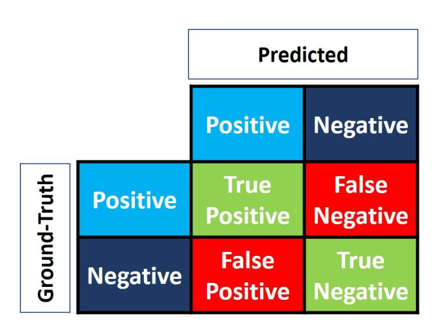
\includegraphics[width=0.8\linewidth]{pictures/Konfusionsmatrix_hs_analysis.png}
    \caption{Darstellung einer Konfusionsmatrix anhand von Annotationen (Ground-Truth) und Vorhersagen (Predicted) gemäß eines XNOR-Gatters}
    \label{fig:Konfusionsmatrix}
    \cite{noauthor_crc-modell_nodate}
\end{figure}


Precision 
\begin{equation}
    Precision = \frac{\mbox{\textit{correctly classified actual positives}}}{\mbox{\textit{everything classified as positive}}} = \frac{TP}{TP + FP}
\end{equation}

Die Präzision beträgt im Idealfall ebenfalls 1,0 und hängt von der Anzahl falsch positiver Ergebnisse ab. Je geringer diese ist, besto besser die Genauigkeit. Präzision und Recall stehen sich in der Form gegenüber, als dass sie ein umgekehrtes Verhältnis haben und in der Regel mit steigender Präzision der Recall abnimmt vice versa.


\begin{equation}
    Recall (\mbox{\textit{True Positive Rate, TPR}}) = \frac{\mbox{\textit{correctly classified actual positives}}}{\mbox{\textit{all actual positives}}} = \frac{TP}{TP + FN}
\end{equation}

Der Recall ist ein Indikator für die Erkennungswahrscheinlichkeit eines Modells, wobei ebenfalls ein Wert von 1,0 = 100\% angestrebt wird. Für die Anwendung an realen Datensätzen mit geringem Aufkommen positiver Ergebnisse bietet diese Berechnung mehr Aussagekraft als die Genauigkeit. Erfasst wird die Fähigkeit eines Modells zur richtigen Identifikation von positiven Instanzen.

\begin{equation}
    \mbox{\textit{FPR (False Positive Rate)}} = \frac{\mbox{\textit{incorrectly classified actual negatives}}}{\mbox{\textit{all actual negatives}}} = \frac{FP}{FP + TN}
\end{equation}

Die Wahrscheinlichkeit eines Fehlalarms, wie die Falsch-Positiv-Rate auch genannt wird, soll im Idealfall bei 0,0 und somit 0 \% liegen. Im Realfall ergibt sich die Aussagekraft aus der Anzahl von tatsächlichen Negativwerte und damit eine entsprechende Instabilität. 

F1-Score
\begin{equation}
    2 * \frac{Precision * Recall}{Precision + Recall}
\end{equation}

Der F1-Score liefert den harmonischen Mittelwert anstelle des arithmethischen aufgrund der stärkeren Gewichtung von großen Unterschieden. Mit niedriger Genauigkeit (Precision) oder Trefferquote (Recall) sinkt das Ergebnis selbst bei einem hohen Gegenwert.  

Im Wesentlichen werden also die Schwächen von Präzision und Recall miteinander verrechnet und darüber ausgewogen, was schwerer zu manipulierendes Resultat bedeutet. 

Accuracy 
\begin{equation}
    Accuracy = \frac{\mbox{\textit{correct classifications}}}{\mbox{\textit{total classifications}}} = \frac{TP + TN}{TP + TN + FP + FN}
\end{equation}

Die Genauigkeit beschreibt den Anteil aller korrekten Klassifizierungen unabhängig von wahr oder falsch. Dies kann bei einer ausgewogenen Verteilung von TP und TN als eine ungefähre Übersicht für die Modellqualität dienen. Im Idealfall würde ein perfektes Modell weder falsch positive noch falsch negative Ergebnisse produzieren, was einer hundertprozentigen Genauigkeit entsprechen würde.

Im Realfall liegen unausgewogene Datensätze vor, bei dem entweder FN oder FP als Fehler überwiegt und damit die Aussagekraft reduziert. Entsprechend würde bei einem seltenen Aufkommen einer Klasse von nur 1\% das Modell in 100\% der Fälle \say{negativ} Vorhersagen, was in 99\% korrekt und dennoch nutzlos wäre. 

Die Kürzel stehen für folgendes: TP = True Positive (wahre Positive), TN = True Negative (wahre Negative), FP = False Positive (falsche Positive) und FN = False Negative (falsche Negative).

Die Wahl fällt hier auf den harmonischen Mittelwert gegenüber des arithmethischen aufgrund der stärkeren Gewichtung von großen Unterschieden. Mit niedriger Genauigkeit (Precision) oder Trefferquote (Recall) wird sinkt das Ergebnis selbst bei einem hohen Gegenwert.  

Intersection over Union
\begin{equation}
    IoU = \frac{|A\cap B|}{|A\cup B|}
\end{equation}
Die Intersection over Union (zu Deutsch: Verhältnis der Schnittmenge zur Vereinigungsmenge, auch genannt Jaccard-Koeffizient) stellt ein Ähnlichkeitsmaß für Vektoren, Mengen und andere Objekte dar. Das dient der Beurteilung der Genauigkeit von Objekterkennungsmodellen und ihrer Optimierung. So definiert in \cite{goodfellow_2016}.

In der Form des Projekts stellt \textbf{IoU} die Schnittmenge der Ground Truth Pixelannotation und Vorhersage geteilt durch die Vereinigungsmenge derselben dar. Je ähnlicher Schnitt- und Vereinigungsmenge desto mehr nähert sich der Wert gleich eins. Während hierbei vollständige Übereinstimmung herrscht, ist diese bei null überhaupt nicht vorhanden. Es handelt sich also um eine prozentuale Gewichtung (?). Die \textbf{mIoU} -> \textbf{mean Intersection over Union} beschreibt den durchschnittlichen IoU über mehrere Objekterkennungen zur besseren Gesamtakkuranz eines Models. Da die Segmentierung pixelweise geschieht, ist der allgemeine Durchschnitt das beste Maß, solange das Objekt selbst keine Rolle spielt. 


\textbf{Quantisierung/Optimierung} für Edge-Geräte ergänzen (z.B. Post-Training Quantization, INT8/FP16, Latenz vs. Genauigkeit, Speicherbedarf; Bezug zu TensorFlow Lite).

Um den Anspruch an die Rechenressourcen zu reduzieren, wird \textbf{Post Training Quantization (PTQ)} eingesetzt. Damit hierbei keine Präzision verloren geht, wird die herkömmliche FP16 Aktivierungsausbreitung auf INT8 komprimiert. Das führt zu etwas g\cite{tensorflowPosttrainingQuantization}

\section{Theoretische Grundlagen}
\subsection{Neuronale Netze - Deep Learning}
Künstliche Intelligenz und Neuronale Netze stellen seit einigen Jahren den Status Quo dar, weswegen diese Technologie jedem ein Begriff sein sollte. Dennoch sei die grundlegende Funktionsweise hier erklärt, um das Basiswissen zu vereinheitlichen: 

Das sogennante \say{Deep-Learning} stellt, wie der Name es bereits andeutet, eine vertiefende Variante des machinellen Lernens dar. Während bei dieser veralteten Form noch Algorithmen definiert werden, die anhand mathematischer Logik Operationen explizit ausführen, werden bei der Tiefenlern-Methode. Mittels Verzerrungen und Gewichtungen des Modells kann das neuronale Netz auf der Basis von maschinellem Lernen optimiert werden, indem die Verknüpfung hinsichtlich ihrer Stärke angepasst werden. Während neuronale Netze und \say{Deep Learning} oft synonym verwendet werden, sind die Begriffe nicht ganz identisch. Per Definition liegt Deep Learning erst ab vier Schichten vor, obwohl moderne neuronale Netze diese Tiefe weit überschreiten.  \cite{goodfellow_2016} \\ \\

\begin{figure}
    \centering
    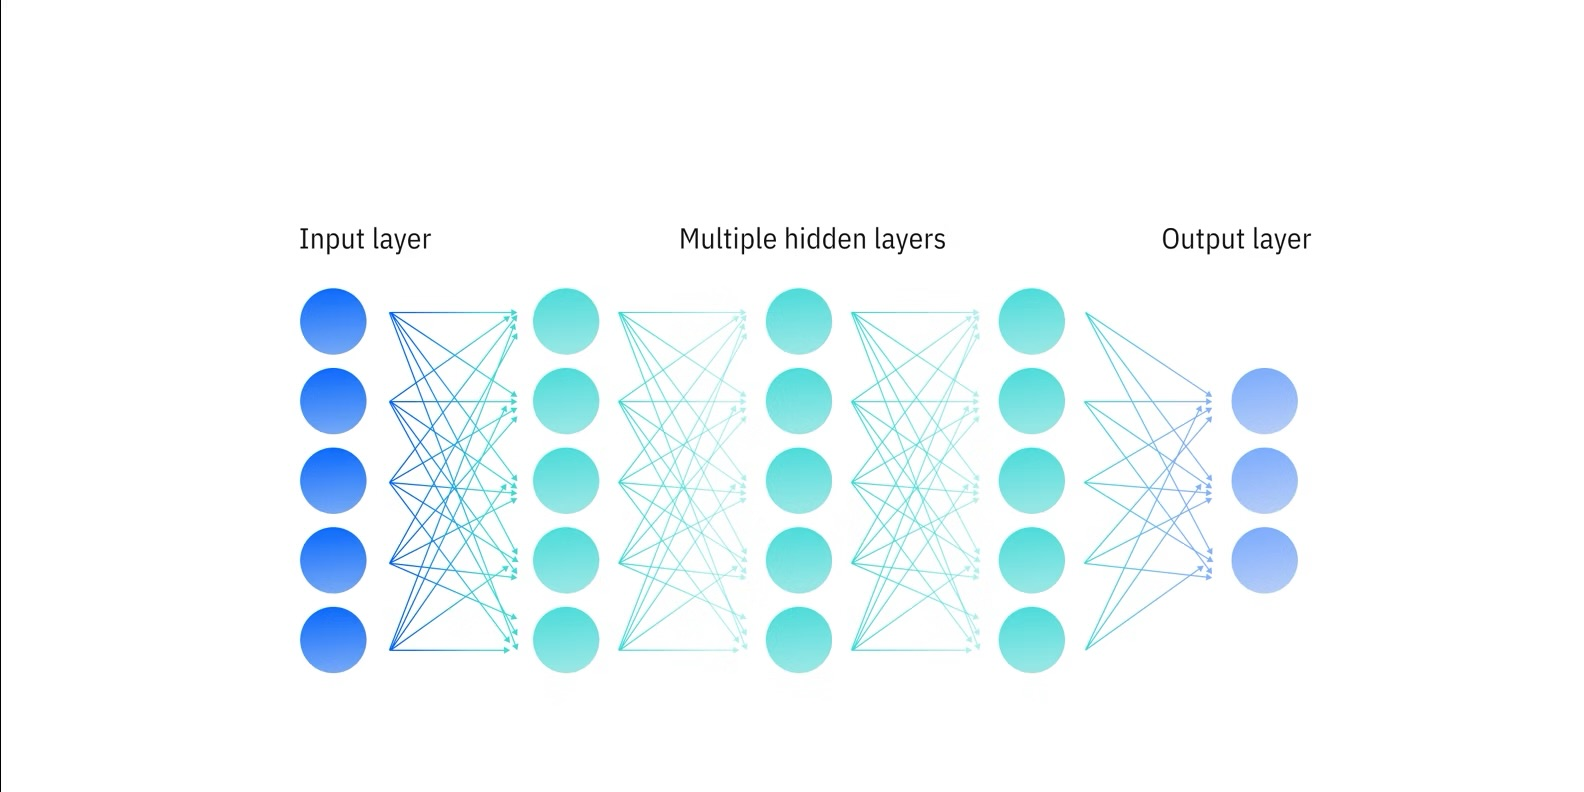
\includegraphics[width=0.5\linewidth]{pictures/deep-neural-network-diagram_2x1.png}
    \caption{}
    \label{fig:neural_network}
\end{figure}

Die unterschiedliche Funktionsweise von maschinellem Lernen und \say{Deep-Learning} lässt sich anhand dieses Gedankenexperiments darstellen: die Daten liegen als einzelne Punkte (x,y) in einem zweidimensionalen Koordinationsystem und sollen mittels Modelltrainings so verarbeitet werden, dass eine Linie diese erfasst. Während der klassische Lösungsansatz in der Definition einer Funktion liegt, die in Linien- oder Kurvenform dieses Ziel erreicht (machinelles Lernen), werden bei dem modernen Ansatz sämtliche Linien durch einzelne Punkte angepasst, rekombiniert und schließlich zu einer Form zusammengefügt. \cite{goodfellow_2016}

Aufgrund ihrer hohen Flexibilität werden neuronal Netze auch als ``universelle Approximatoren'' bezeichnet, da hypothetisch jede Funktion über eine neuronale Netzvereinbarung reproduziert werden kann.



\section{Convolutional Neural Network}

Ein Convolutional Neural Network (CNN oder ConvNet), zu deutsch ein faltbares neuronales Netzwerk, ist ein speziell für die Bild- und Videoverarbeitung ausgelegtes Konzept, was in seinen Grundstrukturen 1979 von Kunihiko Fukushima mit dem \say{Neocognitron} entwickelt und seitdem schrittweise verbessert wurde. 

Namensgebend sind die Convolutional Layer, die auf dem Prinzip der diskreten Faltung basieren. Hierfür wird mittels eines Filterkernels die Eingabe schrittweise verarbeitet und dieses innere Produkt wird an die Neuronen weitergeleitet. Aufgrund der Mehrfachverarbeitung von überlappenden Bereichen zeichnen sich Ähnlichkeiten bei benachbarten Neuronen ab. Das Training der jeweiligen Schicht an Neuronen ist hierbei auf den Inhalt der vorherigen Schicht beschränkt, was sich durch die Ursprünge aus den biologischen rezeptiven Feldern herleitet. Dabei werden im Wesentlichen Informationen aus einem Bereich an Sinnesrezeptoren über ein Neuron verarbeitet, was Vorteile in der biologischen Datenverarbeitung bietet. 
Ein weiterer relevanter Bestandteil sind die geteilten Gewichte sämtlicher Neuronen (shared weights), die eine Grundlage für die Erkennung von Kanten, Ecken und weiteren Basisformen bietet. Auch die jeweilige Intensität in der Detektion kann angepasst werden, was vor allem bei der Kantenerkennung als Grundlage in der Bilderkennung verwendet. 

\begin{figure}
    \centering
    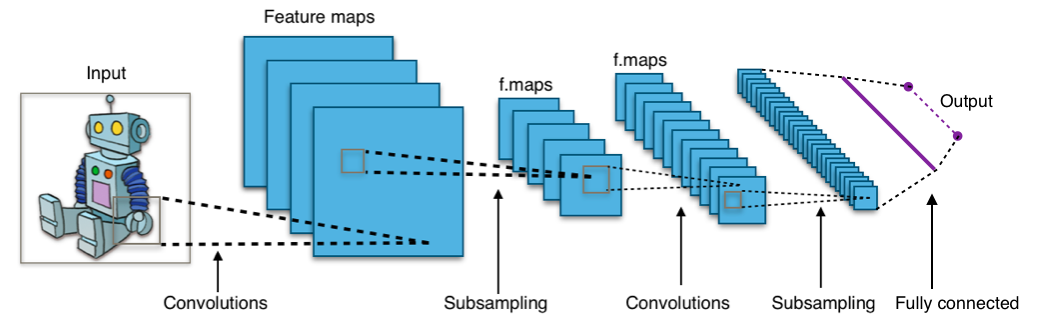
\includegraphics[width=1\linewidth]{pictures/Typical_cnn_wikimedia.png}
    \caption{Verarbeitung der Daten über mehrere Schichten des CNN}
    \label{fig:CNN_Layers}
\end{figure}

Weitergehend werden für gewöhnlich ReLUs und Backpropagation für die Konvertierung des Inputs zum Output verwendet. 
Mittels der Faltungsmatrix wird die regulär eine zwei- bis dreidimensionale Matrix als Input verarbeitet, was zu einer Aktivierung führt. Bei repetitiver Ausführung dieses Schritts zeichnet sich eine Feature Map als Karte dieser Aktivierungen ab. Mit Convolutional Layern werden mehrere dieser datensatzspezifischen Filter gleichzeitig erlernt und dadurch die Erkennung von typischen Merkmalen gestärkt.    

\section{MobileNetV3}

MobileNet ist ein leichtes Convolutional Neural Networks (CNN) von Howard et al das für den Einsatz auf mobilen Endgeräten entworfen wurde und entsprechend geringere Anforderungen im Vergleich zu ähnlichen Modellen aufweist. Ein Kernelement sind die depthwise separable convolutions. Diese ersetzen die konventionellen Convolutional Layer durch ein zweischichtiges System. Einerseits werden räumliche Tiefeninformationen grob und leichtgewichtig bearbeitet sowie zugleich konserviert, während im zweiten Layer eine aufwändigere punktweise 1x1 Faltung vorgenommen wird, die der Generierung von Eigenschaften gilt. Durch diese Trennung sinkt die Anzahl an Parameter und mathematische Operationen, während die Aussagekraft hoch bleibt. 

Verbessert wurde dieses Grundmodell mit Version 2 bei dem inverted residuals und linear bottlenecks eingeführt wurden. Bei invertierten Residuen handelt es sich um eine Möglichkeit des Netzwerks, Aktivierungen früher zu erreichen. Indem eine Verbindung zwischen Anfang und Ende eines Convolutional Blockes geschaffen wird, können Hochskalierungen übersprungen und damit Parameter eingespart werden, was sich für das Training von tiefen Netzen als äußerst effizient herausgestellt hat.   
Andererseits werden hierdurch Leistungseinbußen verursacht, die an anderer Stelle korrigiert werden mit linearen Flaschenhälsen. Dafür werden 1x1 Layer zwischen den restlichen Schichten in die building blocks für In- und Output eingebaut, die die Eingabe auf das Format reduzieren und somit harmonisieren. Die Blöcke der layer transformation bestehen weiterhin aus einer nicht linearen Funktion, was die Vorteile beider Varianten bedeutet.
\cite{}

\begin{figure}[h]
    \centering
    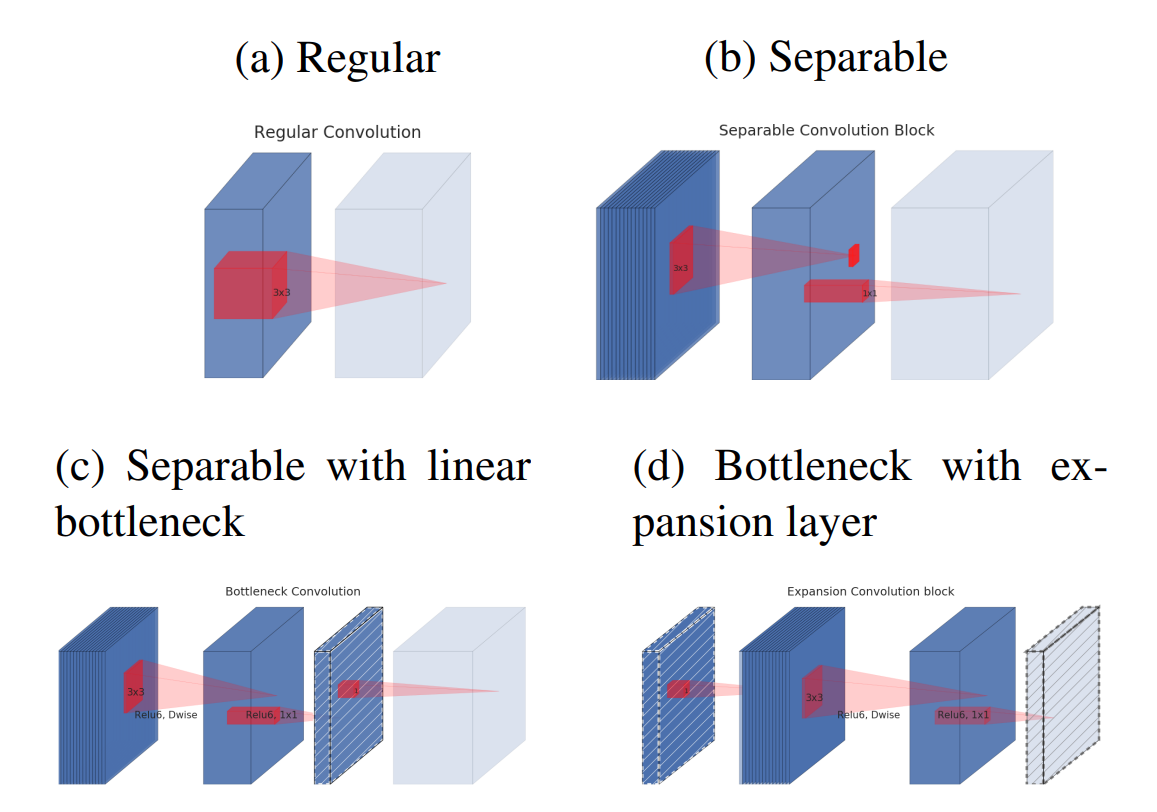
\includegraphics[width=0.6\linewidth]{pictures/MobileNetV2_Convolutions_og_paper.png}
    \caption{Darstellung der unterschiedlichen Varianten von Convolutions mit den Merkmalen von MobileNet}
    \label{fig:convolutions}
\end{figure}

\begin{figure}[]
    \centering
    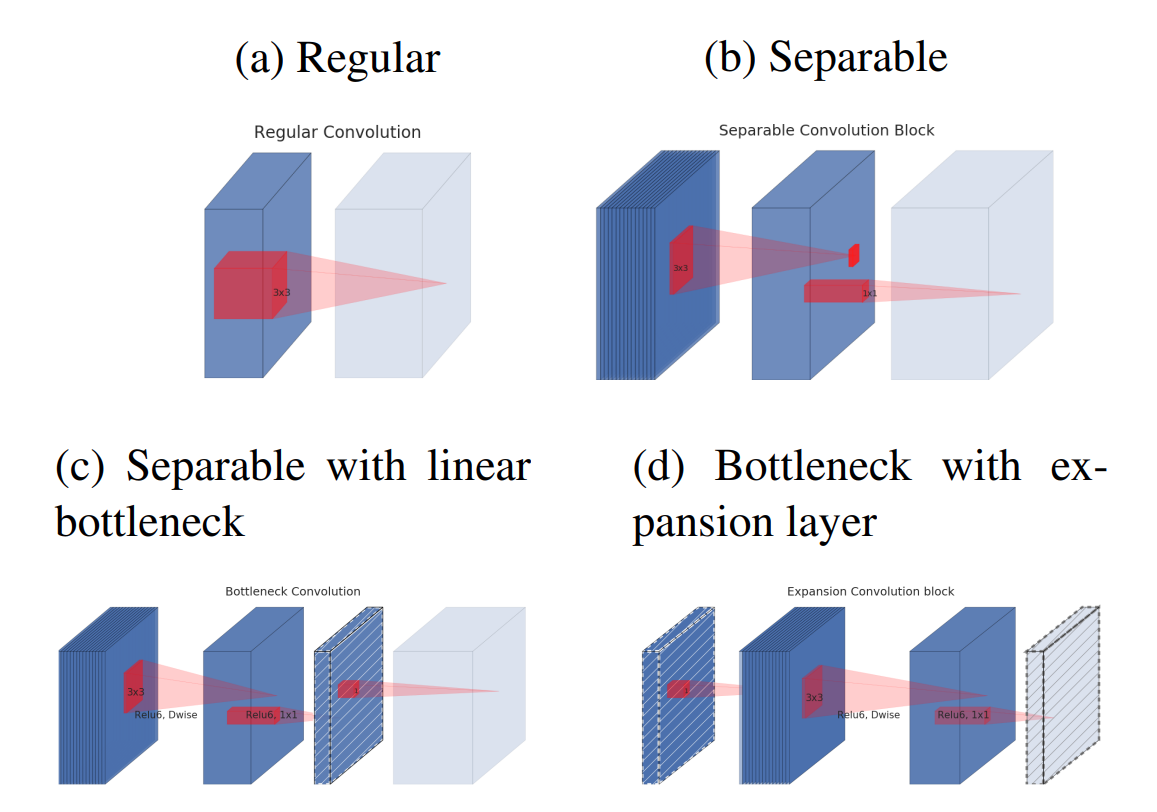
\includegraphics[width=0.8\linewidth]{pictures/MobileNetV2_Convolutions_og_paper.png}
    \caption{Darstellung der unterschiedlichen Varianten von Convolutions mit den Merkmalen von MobileNet}
    \label{fig:convolutions}
\end{figure}

\textbf{Quelle zur Abbildung ergänzen} und korrekt zitieren (\texttt{\textbackslash cite\{...\}}); leere Zitation entfernen, sonst Bibliographiefehler.

Im Rahmen der MobileNet Version V3 wurden die bestehenden ReLUs durch swish nonlinearity Funktionen ersetzt, die eine Kombination aus einfacher und harter Sigmoid-Funktion darstellt. 
Darüber hinaus wurde die Plattformerkennung mittels NAS optimiert, ein Netzwerk-Feintuning durch NetAdapt und Squeeze-and-Excite (SE) Module hinzugefügt.



\section{Zusammenfassung/Bewertung}
Aufgrund der vielseitigen Anforderungen an das Projekt hinsichtlich der Umgebung, Sicherheitsanforderungen und Zeitrahmens stellt ein auf Raspberry Pi 5 basierendes System mit MobileNetV3 unter TF-Lite Runtime die beste Alternative dar. Hiermit gestaltet sich der hochwertigste Trade-Off zwischen Perfomanz, Simplizität und Kosten. Das zugrunde liegende CNN in Kombination mit Semantischer Segmentierung ist zwar eine aufwändigere Form durch die notwendige Pixelannotation, bietet aber Vorteile durch simple Grenzwertbestimmung, die für das Schaltverhalten der Peripherie sinnvoll ist. Der Raspberry stellt durch die Vielfalt an Online-Anleitungen und direkte physische Anbindung per GPIO-Pins den optimalen Kompromiss aus DIY- und Industrielösung dar, ohne einen Mikrocontroller zu benötigen. 


\ldots
% !TEX root = ../Thesis.tex
%%
%%  Hochschule für Technik und Wirtschaft Berlin --  Abschlussarbeit
%%
%% Kapitel 3 - Konzept / Architektur
%%
%%

%\chapter{Konzeption} \label{Konzept}

\section{Test}

Für die Umsetzung einer Wasseroberflächenüberwachung wurden in dieser Arbeit viele Entscheidungen gefällt, die sich konkret mit den limitierenden Faktoren auseinander setzen. Diese sind insbesondere: 

Kritische Infrastruktur
Die Berliner Wasserbetriebe haben als Versorger des Landes Berlin und Umgebung eine große Verantwortung und Sorgfaltspflicht gegenüber den Konsumenten und Nutzern. Auch die Abwasserentsorgung unterliegt dementsprechend strengen Richtlinien, die Auswirkungen auf Arbeitsprozesse genommen haben.
So ist die Wahl eines Air-Gaps in der Hardware als höchste Sicherheitsstufe unmittelbar darauf zurückzuführen. Diese simple Entscheidung hat bereits gravierende Auswirkungen auf unterschiedlichste Lösungsansätze genommen wie das Betreiben eines Zweitrechners zum Überspielen der Daten, die Wahl des Neuronalen Netzes in seinem Aufbau und die Datenerfassung selbst.

\textbf{Ergänzen}: kurzes Sicherheits-/Threat-Model (welche Angreifer/Fehlerszenarien, welche Daten sind sensibel), sowie konkrete Konsequenzen für Betrieb/Updates: wie gelangen Trainingsdaten/Modelle/Logs über den Air-Gap (Medium, Prozess, Verantwortlichkeiten)?

Da das Bilderfassungssystem im Außeneinsatz positioniert ist, ergeben sich umfassende Anforderungen in Anbetracht der physischen Anbindung an die Peripherie, dem Umgang mit Witterungsbedingungen als auch Zuverlässigkeit und Wartungsminimierung. 

Zeit ist immer ein limitierender Faktor, wenn es um die Einarbeitung in ein fachfremdes Thema geht, in dem die Betrachtung von Umständen notwendig ist, mit denen man sich weder selbst noch jemand anderes in dem Bereich bereits auseinandergesetzt hat. Entsprechend sind Design-Entscheidungen dann auch relevant, wenn es um die Planung und Skalierung von Ressourcen geht. So ist bei der Beschaffung von Materialien immer auch mit der Umgebung zu rechnen und der Umfang entsprechend klein zu halten. 

\section{Entwurf des eigenen Lösungskonzepts}


    
\begin{figure}[h]
    \centering
    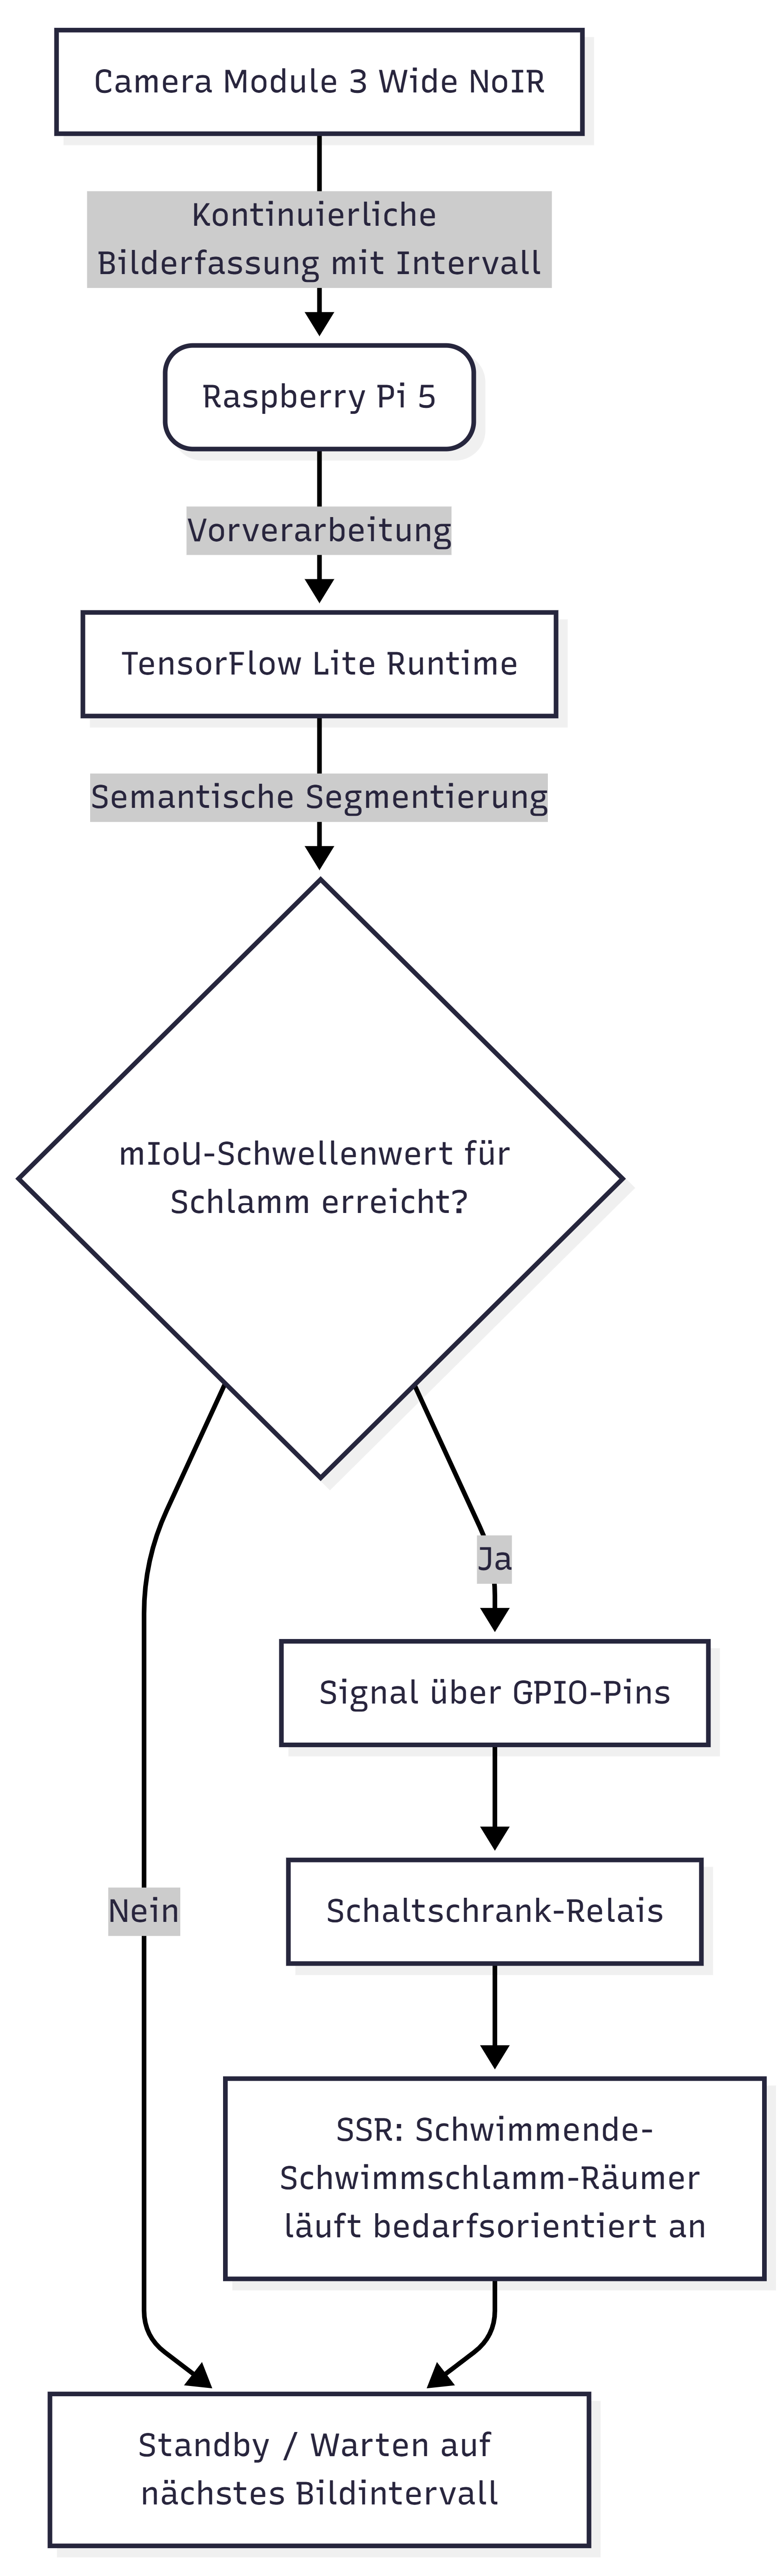
\includegraphics[width=0.4\linewidth]{pictures/Bildverarbeitung.png}
    \caption{Visualisierung der Bildverarbeitungspipeline}
    \label{fig:Bildpipeline}
\end{figure}
    
    




\pagebreak

\textbf{Ausformulieren}: Konzept als durchgängiger Daten-/Steuerungsfluss (Kamera $\rightarrow$ Preprocessing $\rightarrow$ Modell $\rightarrow$ Entscheidung $\rightarrow$ Aktorik). Danach die Entscheidung begründen (Kriterien, Alternativen, warum verworfen). Vorteil/Nachteil-Liste in argumentativen Text überführen und mit Anforderungen verknüpfen.

    


\begin{table}[]
\begin{tabular}{|l|l|l|}
\hline
\textit{\textbf{Komponente}} & \textit{\textbf{Vorteile}} & \textit{\textbf{Nachteile}} \\ \hline
\textbf{Raspberry Pi 5}      & Preiswert                  & Schlechte Skalierbarkeit    \\ \hline
                             & Anpass- und erweiterbar    & Kein Industriestandard      \\ \hline
                             & Perfomant                  & Hoher Wartungsaufwand       \\ \hline
                             & Open Source                & Lokal beschränkt            \\ \hline
                             & Anbindungsmöglichkeit      & Komplexer Systemaufbau      \\ \hline
                             & Lokal trainierbar          &                             \\ \hline
\textbf{Edge-AI Cam}         & Hohe Skalierbarkeit        & Teuer                       \\ \hline
                             & Industriestandard          & Geschlossenes System        \\ \hline
                             & Niedriger Wartungsaufwand  & Externe Ressourcen          \\ \hline
                             & Hoher Stromverbrauch       & Hoher Planungsaufwand       \\ \hline
                             & Netzwerkweit angebunden    &                             \\ \hline
                             & Simple Benutzeroberfläche  &                             \\ \hline
\end{tabular}
\end{table}

\begin{itemize}
\item Darstellung des eigenen Ansatzes, ggf. Abgrenzung von anderen Arbeiten
\item Vorteile
\begin{itemize}
    \item Preiswerter Einplatinencomputer
    \item Gute Anpassungs- und Erweiterungsmöglichkeiten
    \item Hohe Performance
    \item Open Source
    \item Unkomplizierte Anbindung
    \item Lokal trainierbar
\end{itemize}
\item Nachteile
\begin{itemize}
    \item Schlechte Skalierbarkeit
    \item Kein Industriestandard
    \item Hoher Wartungsaufwand
    \item Hoher Stromverbrauch ?
    \item Lokal beschränkt
    \item Geringe Systemeinsicht
\end{itemize}

\end{itemize}
\section{Auswahl/Entwurf der Hardware}

\begin{table}[]
\begin{tabular}{|l|l|l|l|l|l|} \hline
\textbf{Komponente}          & \textbf{Aufgabe}                                       & \textbf{Spezifikation}             & \textbf{CPU}                     & \textbf{RAM} \\ \hline 
ThinkPad T14 & Internet & 256 GB SSD                            & Intel i5-1135G7         & 32 GB 2700 MHz   \\ \hline
Pro Rugged 14  & Coding                          & 2 TB SSD                              & Intel Ultra 5 125U x 12 & 32 GB 5600 MHz \\ \hline
Pi 5      & Verbindung                           & 64 GB SD-Karte                        & Broadcom BCM2712        & 8 GB 4267 MHz \\ \hline
Camera Module 3     & Peripherie                                    & Wide-NoIR & -                       &   - \\ \hline
\end{tabular}
\end{table}


Für die praktische Umsetzung des Edge-Computing-Systems zur Wasseroberflächenüberwachung wird eine dedizierte Hardware-Architektur benötigt, die den strengen Vorgaben der Air-Gap-Umgebung sowie den harschen Bedingungen vor Ort am Nachklärbecken gerecht wird. Die Infrastruktur teilt sich hierbei in drei primäre Rechenleistungen und eine optische Erfassungskomponente auf:  Als primäres Arbeitsgerät für den administrativen und netzwerkgebundenen Teil der Arbeit kommt ein Lenovo ThinkPad T14 zum Einsatz. Aufgrund der Sicherheitsrichtlinien der Berliner Wasserbetriebe dient dieses Endgerät ausschließlich als Schnittstelle zur Außenwelt, um die notwendige Internetanbindung für die globale Informationsbeschaffung zu gewährleisten. Darüber hinaus wird dieses System für die cloudbasierte oder lokale Textdokumentation der Ausarbeitungen genutzt.  Für die rechenintensiven Prozesse des Projekts wird ein robustes Notebook vom Typ Dell Latitude Pro Rugged herangezogen. Dieses System agiert innerhalb der Air-Gap-Umgebung komplett offline. Seine Hauptaufgaben liegen im lokalen Training des Neuronalen Netzes, der direkten Kommunikation und Konfiguration des Edge-Geräts via Kabelverbindung sowie der anschließenden mathematischen und statistischen Auswertung der Testergebnisse.  Die eigentliche Ausführung des KI-Modells direkt am Prozess (Edge-Computing) übernimmt ein Raspberry Pi 5. Dieser zeichnet sich durch eine hohe Recheneffizienz bei geringer Leistungsaufnahme aus und ist für die kontinuierliche Datenerfassung der Bildströme sowie die anschließende Peripheriesteuerung des Schwimmenschlamm-Räumers (SSR) verantwortlich.  Die optische Datenerfassung erfolgt über das Raspberry Pi Camera Module 3 Wide NoIR. Die Wahl fiel explizit auf die NoIR-Variante (No Infrared), um über externe Infrarotscheinwerfer eine lückenlose Nachtsicht und Ausleuchtung der Wasseroberfläche zu realisieren. Das Weitwinkelobjektiv (Wide) garantiert hierbei einen maximalen Erfassungswinkel, um die relevanten Bereiche des Nachklärbeckens optimal abzubilden. Zur Reduktion von störenden Lichtreflexionen und Spiegelungen auf der Wasseroberfläche wird die Optik zudem durch einen dedizierten Polarisationsfilter ergänzt.

\section{Auswahl/Entwurf der Software}
Parallel zur Hardware-Struktur erfordert das System eine harmonisierte Software- und Betriebssystemlandschaft, die den Offline-Betrieb und den Entwicklungsprozess lückenlos unterstützt.


\subsection{Betriebssysteme}

Auf den jeweiligen Hardwarekomponenten kommen drei differenzierte Betriebssysteme zum Einsatz:
Das \textit{Lenovo ThinkPad T14} wird unter \textbf{Windows 11 Enterprise} betrieben, was den Unternehmensstandards entspricht und eine sichere Verbindung zu den internen und externen Netzwerken erlaubt.
Auf dem \textit{Dell Pro Rugged} wird die Linux-Distribution \textbf{Linux Mint} mit der \textbf{Cinnamon-Benutzeroberfläche} eingesetzt. Diese Wahl begründet sich in der hohen Stabilität, der exzellenten Unterstützung für Entwicklerwerkzeuge und der Ressourceneffizienz im Offline-Betrieb.
Als Betriebssystem für die Edge-Plattform (Raspberry Pi 5) wird das offizielle, Debian-basierte \textbf{Raspberry Pi OS} verwendet, da dieses eine native Treiberunterstützung für das genutzte Kameramodul und die GPIO-Schnittstellen bietet.


\subsection{Softwarekomponenten nach System}

    


\begin{enumerate}
    \item \textbf{Lenovo Thinkpad T14:}
    Für die wissenschaftliche Ausarbeitung der Arbeit wird das kollaborative Online-LaTeX-System \textbf{Overleaf} genutzt. Die Erstellung der Ground-Truth-Daten und die manuelle Annotation der Bilddatensätze erfolgt über das webbasierte Tool \textbf{CVAT} (Computer Vision Annotation Tool).
    \item \textbf{Dell Pro Rugged:}
    Die lokale Softwareentwicklung und das Skript-Debugging werden in der Entwicklungsumgebung \textbf{Visual Studio Code} durchgeführt. Zur softwareseitigen Umsetzung der KI-Infrastruktur bildet die Python-Distribution \textbf{Anaconda} das Fundament, welche das Paket- und Environment-Management im Offline-Modus erleichtert. Das Training und die Evaluierung des semantischen Segmentierungsmodells basieren auf den Deep-Learning-Frameworks \textbf{Tensorflow} und \textbf{Keras}, während \textbf{Tensorboard} zur visuellen Analyse und Überwachung der Trainingsmetriken (wie Loss und IoU) eingesetzt wird. Bildverarbeitungsoperationen sowie mathematische Matrixoperationen werden über die Bibliotheken \textbf{OpenCV} und \textbf{NumPy} händisch implementiert.
    \item \textbf{Raspberry Pi 5:}
    Um den KI-Inferenzprozess auf dem Edge-System so performant und ressourcenschonend wie möglich zu gestalten, wird auf dem Kleinstcomputer auf die vollständige Tensorflow-Bibliothek verzichtet. Stattdessen kommt exklusiv die schlanke \textbf{TensorFlow Lite Runtime} (\textit{TFlite Runtime}) zum Einsatz, welche für die ressourceneffiziente Echtzeit-Segmentierung des Bildmaterials optimiert ist.
\end{enumerate}



\begin{lstlisting}[caption=Code zur Umwandlung von .mp4 zu .png]
import cv2
import os

video_path = "/home/oem/Desktop/BIldmaterial/IMG_0002.MOV"
output_dir = "extracted_images"
interval_seconds = 1  

if not os.path.exists(output_dir):
    os.makedirs(output_dir)

cap = cv2.VideoCapture(video_path)
fps = cap.get(cv2.CAP_PROP_FPS)
interval_frames = int(fps * interval_seconds)

count = 0
image_id = 0

while cap.isOpened():
    ret, frame = cap.read()
    if not ret: break
    
    if count % interval_frames == 0:
        cv2.imwrite(f"{output_dir}/img_{image_id:04d}.png", frame)
        image_id += 1
    count += 1

cap.release()
print(  )
print(f"Fertig! {image_id} Bilder exportiert.")
\end{lstlisting}

\begin{lstlisting}[caption=Code zur Maskengenerierung in]
    import cv2
import numpy as np
import os
from os import path
from os import listdir
from cv2 import cvtColor
from cv2 import imread

input_folder = '/home/oem/Desktop/CVAT/extracted_images'
output_folder = '/home/oem/Desktop/CVAT/masked_images/SegmentationClass'
num_classes = 2
register_file = '/home/oem/Desktop/CVAT/masked_images/Segmentation/default.txt'

os.makedirs(output_folder, exist_ok=True)

os.remove(register_file)

def auto_annotate(image_path):
    img = cv2.imread(image_path, flags=cv2.IMREAD_COLOR)
    hsv = cv2.cvtColor(img, cv2.COLOR_BGR2HSV)

    lower_blue = np.array([20, 20, 20])
    upper_blue = np.array([255, 255, 255])

    contra_upper_blue = np.array([0, 0, 0])

    mask3 = cv2.inRange(hsv, lower_blue, upper_blue)
    mask4 = cv2.inRange(hsv, contra_upper_blue, lower_blue)

    #Rauschen filter - optional
    kernel = np.ones((5,5), np.uint8)
    mask3 = cv2.morphologyEx(mask3, cv2.MORPH_OPEN, kernel)

    #Hintergrund-Klasse
    combined_mask = np.zeros(mask3.shape, dtype=np.uint8)

    combined_mask[mask3 > 0] = 1 
    return combined_mask

    base_name = os.path.basename(image_path).split('.')[0]

    #Konvertierung zu numerischen Arrays
    cv2.imwrite(os.path.join(output_folder, f"{base_name}_mud.png"), mud_mask.astype(np.uint))
    cv2.imwrite(os.path.join(output_folder, f"{base_name}_water.png"), water_mask.astype(np.uint))

    return mud_mask, water_mask

for images in os.listdir(input_folder):
    mask = auto_annotate(os.path.join(input_folder, images))
    out_name = (images)
    
    name_wo_extension = os.path.splitext(images)[0]

    with open(register_file, "a") as f:
        f.write(name_wo_extension + "\n") 
        
        cv2.imwrite(os.path.join(output_folder, out_name), mask)
        
with open(register_file) as lines:
    names = list(lines)
names.sort()
print(names)


\end{lstlisting}

%\subsection{Entwurf von Lösungsmodulen}





% !TEX root = ../Thesis.tex
%%
%%  Hochschule für Technik und Wirtschaft Berlin --  Abschlussarbeit
%%
%% Kapitel 3.5 - Vorarbeit
%%
%%

\chapter{Analyse der Air-Gap-Arbeitsumgebung und Tool-Chain} \label{Vorarbeit}



\section{Übersicht}
Vor Beginn der Bachelorarbeit wurde ein dreimonatiges Praktikum absolviert, was sich mit essentiellen Punkten zur Grundlagenbildung auseinander gesetzt hat. 

\subsection{Einführung in das Unternehmen}
Im Rahmen des Praktikums fand an erster Stelle eine Einführung in das Unternehmen selbst statt. So wurden Einblicke in die Organisationsstruktur und einzelne Abteilungen sowie Standorte gegen. Hierzu zählen unter anderem die technische Zentrale am Werner-Voß-Damm, wo der Großteil der Zeit verbracht wurde. Hier fand auch der Einblick in das operative Geschäft in Form von wöchentlichen Teamleitertreffen statt, die insbesondere zum Einsehen in die Tätigkeiten von TS-E (Technischer Service - Elektrotechnik) geeignet waren. 

Ein weiterer Primärstandort war das Klärwerk Waßmannsdorf, in dem ebenfalls ein Großteil der Zeit verbracht wurde. Hier konnten die direkten verfahrenstechnischen Begebenheiten hautnah erlebt und inspiziert werden, was zur Grundlagenbildung enorm beigetragen hat. Das Pilotprojekt findet ebenfalls an diesem Standort statt, was eine hohe Auseinandersetzung mit der Lokalität erforderlich macht.  

%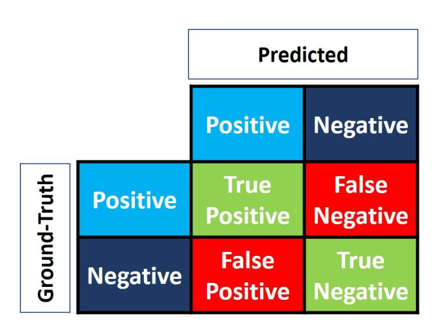
\includegraphics[]{pictures/Konfusionsmatrix_hs_analysis.png}
\subsection{Recherche und Themenfindung}

Im Rahmen der Recherche 

\subsection{Planung und Umsetzung}

Aufgrund der hohen Sicherheitsanforderungen der BWB im Rahmen der Abwasserentsorgung der kritischen Infrastruktur eines Klärwerks, bestehen grundsätzliche Vorgaben zum Arbeiten im Air Gap. Diese waren auch für dieses Projekt von Relevanz, da sämtlich Arbeitsprozesse und Lösungen entsprechend zugeschnitten werden mussten, um lokal und komplikationsarm ausführbar zu sein. Sämtliche Methoden und Lösungen sind so oder in abgewandelter Form auch für die Bachelorarbeit notwendig gewesen. 

\begin{figure}[H]
    \centering
    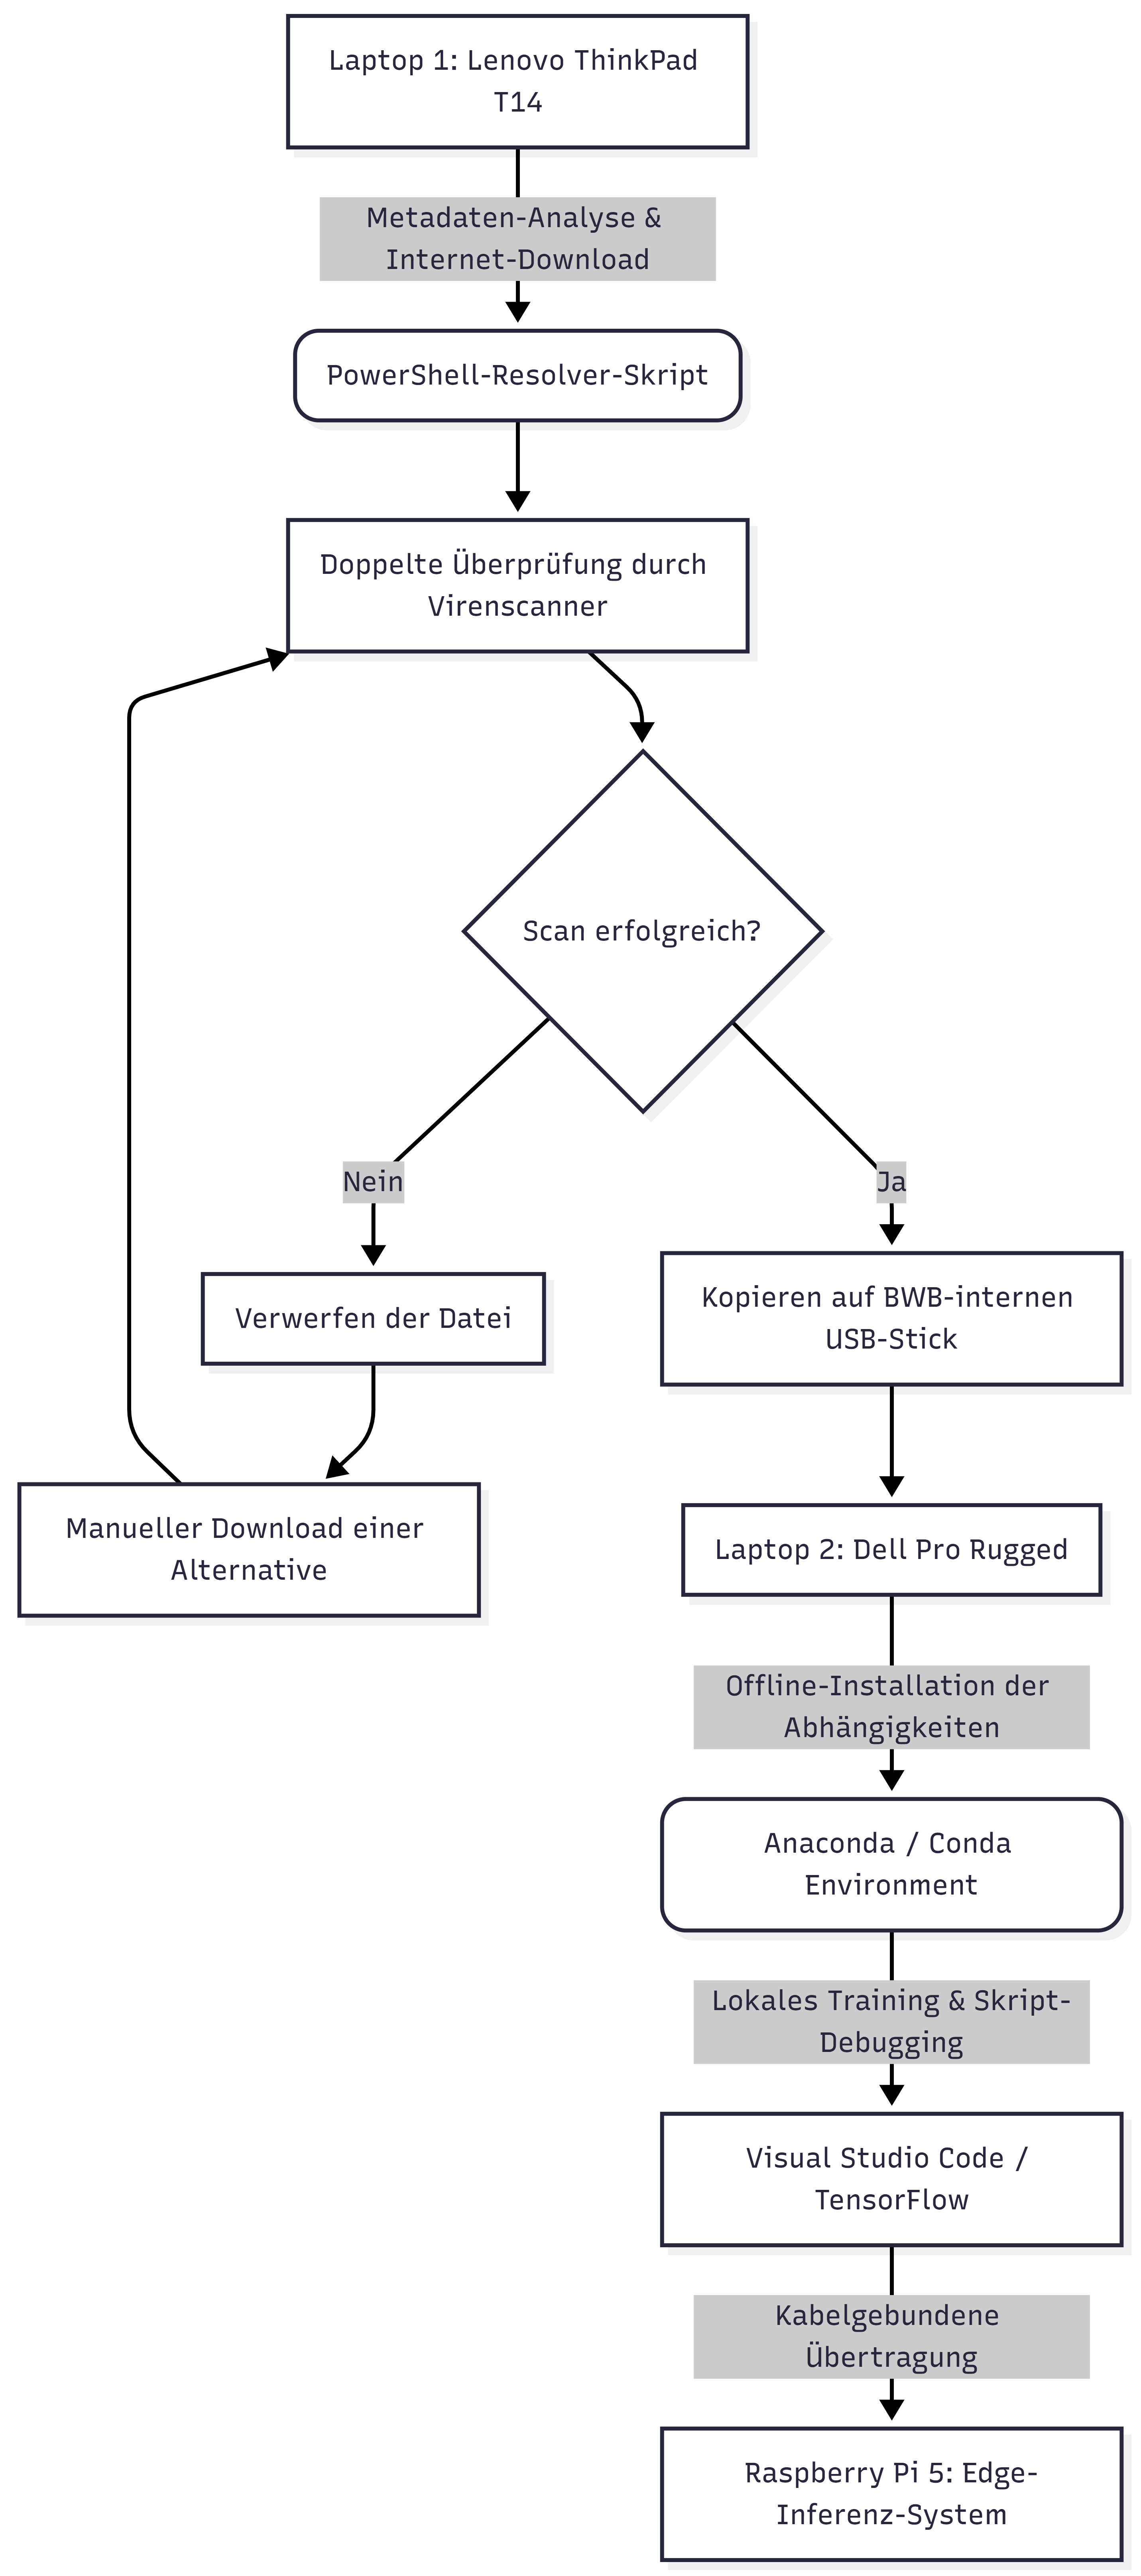
\includegraphics[width=0.5\linewidth]{pictures/Workflow.png} 
    \caption{Darstellung des Air Gaps der Arbeitsumgebung}
    \label{fig:airgap}
\end{figure}

Dieser Air Gap besteht aus zwei von den BWB zugewiesenen Laptops und einem unverschlüsselten USB-Stick. Laptop 1, ein Lenovo ThinkPad T14 liegt ohne Adminrechte und mit Windows 11 vor, um einen Internetzugang herzustellen. Auf Laptop 2 herrschen uneingeschränkte Administratorrechte, aber keine Anbindung an ein internetfähiges Netz. Dieser Laptop ist auch für die Kommunikation mit dem Raspberry PI vorgesehen. Die strikte Vorgabe besagt, dass sämtliche zu beziehenden Dateien für Laptop 2 von Laptop 1 heruntergeladen, per Virenscanner doppelt überprüft und dann auf Laptop 2 kopiert werden. Der USB-Stick ist zudem nur für die Kommunikation zwischen den firmeneigenen Endgeräten zulässig. \\ \\

Dieser Aufbau bringt vielseitige Herausforderungen mit sich, die im Alltag sonst nicht auftreten würden. So wurde auf Laptop 2 die umfassendeste Variante von Linux Mint installiert, um den Anteil an Grundfunktionen zu maximieren und den Umfang an aufwendig zu ladenden Programmen zu minimieren. Dieses Problem hätte sich grundsätzlich durch einen Endgerät mit identischem Betriebssystem lösen lassen, was hier aufgrund der Sicherheitsvorkehrungen nicht möglich war. Die Website PYPI stellt die meisten Installationsdateien mit entsprechender Versionhistorie zur Verfügung.
Mittels eines Skripts wurden die erforderlichen Abhängigkeiten (requires-dist) von Wheel-Dateien aus der METADATA ausgelesen. Hierdurch wurden Informationen wie benötigte Python- und Programmversion einer einzelnen .whl Datei oder einem Ordner ausgelesen. Mit weiteren Spezifikationen im Skript konnten die Downloads dann für die Zielplattform angepasst und iterativ gestalten werden, damit sämtliche Subdependencies aufgelöst werden konnten. Nicht zuletzt wurden herunterzulandende Inhalte mit den im Ordner vorhandenen abgeglichen um Dopplungen zu vermeiden.\\ \\



\begin{lstlisting}[caption=Powershell-Skript zum Download von Wheel Dateien]
$Path           = ".\" # Datei ODER Ordnerpfad
$DownloadDir    = ".\"
$TargetPython   = "Python_Version"
$Platform       = "Platform_Variante"
$MaxThreads     = Anzahl_Threads  # Erhoeht fuer maximale Auslastung

[Net.ServicePointManager]::SecurityProtocol = [Net.SecurityProtocolType]::Tls12
Add-Type -AssemblyName System.IO.Compression.FileSystem

if (!(Test-Path $DownloadDir)) { New-Item -ItemType Directory -Path $DownloadDir | Out-Null }
$GlobalDownloaded = [Hashtable]::Synchronized(@{})
$TotalBytesToDownload = [long]0

function Format-Size ([long]$bytes) {
    if ($bytes -gt 1GB) { return "{0:N2} GB" -f ($bytes / 1GB) }
    return "{0:N2} MB" -f ($bytes / 1MB)
}

function Get-DependenciesFromWheel {
    param($Whl)
    $deps = @()
    try {
        $zip = [System.IO.Compression.ZipFile]::OpenRead($Whl)
        $meta = $zip.Entries | Where-Object { $_.FullName -match "METADATA$" }
        if ($meta) {
            $r = New-Object System.IO.StreamReader($meta.Open())
            while ($l = $r.ReadLine()) { if ($l -match "^Requires-Dist:\s*([^;]+)") { $deps += $Matches[1].Trim() } }
            $r.Close()
        }
        $zip.Dispose()
    } catch {}
    return $deps | Select-Object -Unique
}

$RunspacePool = [RunspaceFactory]::CreateRunspacePool(1, $MaxThreads)
$RunspacePool.Open()
$Jobs = New-Object System.Collections.Generic.List[Hashtable]

function Queue-Download {
    param($RawDep)
    $name = ($RawDep -split "[\s;>=<\[,! ]")[0].ToLower().Trim()
    if ([string]::IsNullOrWhiteSpace($name) -or $GlobalDownloaded.ContainsKey($name)) { return }
    
    $PkgKey = $name.Replace(".","_")
    if (Get-ChildItem $DownloadDir | Where-Object { $_.Name.ToLower().Replace(".","_").StartsWith($PkgKey + "-") }) { 
        $GlobalDownloaded[$name] = $true; return 
    }

    $GlobalDownloaded[$name] = $true
    $targetV = $null
    if ($RawDep -match "==\s*([0-9\.]+)") { $targetV = $Matches[1].TrimEnd('.') }

    $ScriptBlock = {
        param($PkgName, $SpecificVersion, $Dir, $Target, $Platform)
        try {
            $api = Invoke-RestMethod "https://pypi.org/pypi/$PkgName/json"
            $v = if ($SpecificVersion) { $SpecificVersion } else { $api.info.version }
            $rel = $api.releases.$v
            if (!$rel) { $v = $api.info.version; $rel = $api.releases.$v }

            $valid = $rel | Where-Object { $_.filename -match "\.whl$" -and $_.filename -notmatch "macosx|win|aarch64" }
            $best = $valid | Where-Object { $_.filename -match "cp$Target" -and $_.filename -match $Platform }
            if (!$best) { $best = $valid | Where-Object { $_.filename -match "py3-none" -and $_.filename -match $Platform } }
            if (!$best) { $best = $valid | Where-Object { $_.filename -match "py3-none-any" } }
            
            if ($best) {
                $file = $best[0]
                $path = Join-Path $Dir $file.filename
                (New-Object System.Net.WebClient).DownloadFile($file.url, $path)
                return @{ Name = $PkgName; Size = $file.size; File = $file.filename; Deps = $api.info.requires_dist }
            }
        } catch { return $null }
    }

    $PS = [PowerShell]::Create().AddScript($ScriptBlock)
    .AddArgument($name).AddArgument($targetV).AddArgument($DownloadDir)
    .AddArgument($TargetPython).AddArgument($Platform)
    $PS.RunspacePool = $RunspacePool
    $Jobs.Add(@{ PS = $PS; Handle = $PS.BeginInvoke() })
}

# --- AUTOMATISCHE WEICHENSTELLUNG ---
Write-Host "`n>>> INITIALISIERE ANALYSE..." -ForegroundColor Cyan

if (Test-Path $Path -PathType Container) {
    Write-Host "[i] Modus: ORDNER-SCAN ($Path)" -ForegroundColor Gray
    Get-ChildItem $Path -Filter "*.whl" | ForEach-Object {
        $name = ($_.Name -split "-")[0].ToLower().Replace(".","_")
        $GlobalDownloaded[$name] = $true
        Get-DependenciesFromWheel $_.FullName | ForEach-Object { Queue-Download $_ }
    }
} else {
    Write-Host "[i] Modus: EINZELDATEI-SCAN ($Path)" -ForegroundColor Gray
    Get-DependenciesFromWheel $Path | ForEach-Object { Queue-Download $_ }
}

# --- REKURSIVER TURBO-LOOP ---
while ($true) {
    $running = $Jobs | Where-Object { $_.Handle.IsCompleted -eq $false }
    $finished = $Jobs | Where-Object { $_.Handle.IsCompleted -eq $true -and $_.Processed -ne $true }

    foreach ($j in $finished) {
        $res = $j.PS.EndInvoke($j.Handle)
        if ($res) {
            [System.Threading.Interlocked]::Add([ref]$TotalBytesToDownload, $res.Size) | Out-Null
            if ($res.Deps) { foreach ($nd in $res.Deps) { Queue-Download $nd } }
            Write-Host "`r  [DONE] $($res.File) ($(Format-Size $res.Size))" -ForegroundColor Green
        }
        $j.Processed = $true
    }

    $localSum = (Get-ChildItem $DownloadDir | Measure-Object -Property Length -Sum).Sum
    if (!$localSum) { $localSum = 0 }
    $perc = if ($TotalBytesToDownload -gt 0) { [Math]::Min(100, ($localSum / $TotalBytesToDownload) * 100) } else { 0 }

    Write-Host -NoNewline ("`rFortschritt: $(Format-Size $localSum)) ($ | Aktiv: $($running.Count)   ") -ForegroundColor Yellow

    if ($running.Count -eq 0 -and $finished.Count -eq 0) { 
        Start-Sleep -Seconds 1
        if (($Jobs | Where-Object { $_.Handle.IsCompleted -eq $false }).Count -eq 0) { break }
    }
    Start-Sleep -Milliseconds 400
}

$RunspacePool.Close()
Write-Host "`n`n--- FERTIG! ---" -ForegroundColor Cyan
Pause
\end{lstlisting}

\begin{figure}[H]
    \centering
    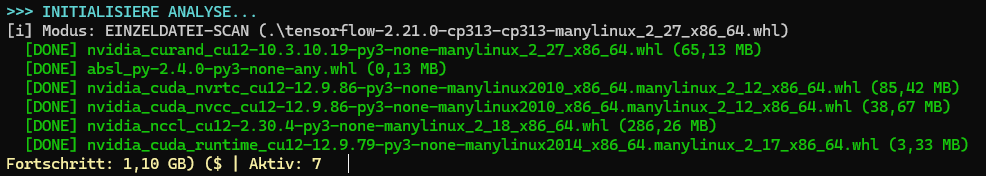
\includegraphics[width=1\linewidth]{pictures/Screenshot_Powershell_Skript.png}
    \caption{Ausführung des Powershell Skript anhand des Beispiels von Tensorflow}
    \label{fig:powershell}
\end{figure}

Wie in \ref{fig:powershell} sichtbar, durchläuft das Skript anhand einer Einzeldatei sämtlich Requires und lädt diese in der passenden Variante parallel über mehrere Threads herunter, damit bei den großen Datenmengen von insbesondere Nvidia Programmen keine überdimensionierten Laufzeiten entstehen. Außerdem wird die Größe des Zielordners und eine Übersicht die Anzahl laufender Prozesse gegeben. Falls die Anforderungen an die Dateiversionen nicht erfüllt werden können, werden stattdessen die none-any-Varianten geladen. Eine vollständige Automatisierung konnte so nicht stattfinden, weswegen einzelne Abhängigkeiten dennoch manuell geladen wurden, aber im Vergleich zur händischen Downloads stellt es trotzdem eine enorme Vereinfachung dar und kann zudem für die Installation des Raspberry PI wiederverwendet werden. \\ \\

Im Rahmen der Arbeit wurden drei unterschiedliche Environments von venv, über Miniconda zu Conda selbst hin vorgenommen. Während Miniconda bereits angenehme Arbeitsweisen ermöglichte, fiel die Wahl letztendlich auf Conda aufgrund preinstalls, da die Anzahl zu installierender Pakete hierdurch deutlich sank. Insbesondere Programme wie PIP wiesen größere Schwierigkeiten auf, da eine Offline-Installation so nicht vorgesehen ist. Der Umschwung auf das umfangreichere Anaconda ermöglichte die problemlosere Installation der weiteren requires, was auch als Option für den Raspberry Pi offen bleibt und nur an Schwierigkeiten mit der Performanz scheitern könnte. \\ \\



ARBEIT IM ENVIRONMENT --> Conda (PIP)


conda activate mud \\ 
pip install program --no-index find-links . 

\section{Produktwahl}

\begin{table}[]
    \centering
    \begin{tabular}{|l|l|}
    \hline
    \textit{\textbf{Name}}                                & \textbf{Raspberry Pi 5}                                  \\ \hline
    \textit{\textbf{Processor (CPU)}}                            & ARM Cortex-A72 quad-core processor with 1.5GHz frequency \\ \hline
    \textit{\textbf{RAM}}
    & 8GB LPDDR4                                               \\ \hline
    \textit{\textbf{Graphics (GPU)}}                             & VideoCore VI GPU, supports 4K                            \\ \hline
    \textit{\textbf{Wireless Connectivity}} & Wi-Fi 5, Bluetooth 5.0                                   \\ \hline
    \textit{\textbf{USB Ports}}                                  & 4 USB 2.0 ports, 1 USB 3.0 port                          \\ \hline
   \textit{\textbf{Ethernet}}                                   & 10/100 Mbps Ethernet                                     \\ \hline
    \textit{\textbf{Storage}}                                    & microSD (no support for internal SSD or eMMC)            \\ \hline
    \textit{\textbf{Camera Support}}                             & CSI-2 port for camera attachment                         \\ \hline
    \textit{\textbf{Power Efficiency}}                           & Average power consumption, optimized for long-term use   \\ \hline
    \textit{\textbf{GPIO Ports}}                                 & 40 programmable GPIO pins                                \\ \hline
    \textit{\textbf{Size \& Design}}                             & Standard design with size of 88x58mm                     \\ \hline
    \textit{\textbf{Price (Estimated)}}                          & Approximate price of 180€ for the advanced model             \\ \hline                              
    \end{tabular}
    \caption{Übersicht der Eigenschaften eines Raspberry Pi 5}
    \label{tab:Eigenschaftstabelle}
\end{table}


% !TEX root = ../Thesis.tex
%%
%%  Hochschule für Technik und Wirtschaft Berlin --  Abschlussarbeit
%%
%% Kapitel 4 - Implementierung
%%
%%

\chapter{Implementierung} \label{Implementierung}

\section{Aufbau der Implementierung}

\textbf{Ergänzen}: detaillierte Implementierungsbeschreibung (Hardware-Verdrahtung/Stromversorgung/Schutzgehäuse, Kamera+IR+Polfilter, GPIO/Aktorik-Anbindung). Schaltplan/Blockschaltbild als Abbildung einfügen und im Text referenzieren.

DARSTELLUNG SCHALTUNG

\section{Montage/Vorrichtung}

Im Anwendungsbereich eines Klärwerks ist im Rahmen der kritischen Infrastruktur eine konkrete Planung der benötigten Vorrichtung notwendig, was entsprechend in Absprache mit der Abteilung TS-E/M/Was, deren Spezialisierung in der Montage besteht. Hierfür wurde eine Profilschiene aus Aluminium dahingehend umgebaut, dass eine Fassung für die Reeling des Nachklärbeckens geschaffen wurde, über die sie eingehakt werden kann. Zusätzlich verfügt dieser "Arm" über ein Gelenk, was auch bei eingebauter Vorrichtung die Anpassung des Neigungswinkels ändert und somit indirekt den Kamerawinkel modifiziert. Das ist für Testzwecke notwendig um den Winkel mit der geringsten Spiegelung für das Kameramodul zu ermitteln. \\ \\

\textbf{Technische Zeichnung}/Foto der Vorrichtung ergänzen (Maße, Material, Befestigungspunkte, Neigungswinkelbereich). Zusätzlich: Witterungsschutz, Kabelmanagement, Zugriff für Wartung/Reinigung beschreiben.
TECHNISCHE ZEICHNUNG \\ \\

PROTOKOLL \\ \\
% !TEX root = ../Thesis.tex
%%
%%  Hochschule für Technik und Wirtschaft Berlin --  Abschlussarbeit
%%
%% Kapitel 5 - Tests
%%
%%

\chapter{Tests} \label{Tests}


\section{Herleitung von Test-Cases}
\textbf{Testmethodik} ausformulieren: Testziele/Hypothesen, Testfälle, Akzeptanzkriterien, Messdauer, Messmittel, sowie Trennung von (a) ML-Evaluierung (mIoU, Precision/Recall, qualitative Beispiele) und (b) Systemtests (Latenz/FPS, Stabilität, Ausfälle, Wartung).
Testen auf: \\
Einsparungen im Stromverbrauch \\
Zuverlässigkeit der Ergebnisse \\
Resilienz/Wartungsintensität im Alltagsbetrieb \\

\subsection{Funktionale Tests}

Als Aufnahme des Ist-Zustands wurde der Durchflussstrom mittels einer Strommesszange ermittelt, anhand des Typenschilds technische Eckdaten erfasst und die Leistung berechnet. Dieser Wert gilt als Grundlage für den Vorher-/Nachhervergleich und damit als Übersicht für die einzusparende Leistung an dem exemplarischen Nachklärbecken bei Umstieg von einer blinden timer-gesteuerten Lösung im Unterschied zu einer bedarfsorientieren. \\ \\

Dieser prototypische Test soll Aussagekraft darüber liefern, inwieweit sich die Skalierung des erdachten Systems lohnen kann und welche Ersparnisse sich daraus in Bezug auf Betrieb, Strom und Personal ergeben.

\begin{figure}[h]
    \centering
    \begin{tabular}{c|c}
         &  \\
         & 
    \end{tabular}
    \caption{Leistungsberechnung Ist-Zustand}
    \label{fig:placeholder}
\end{figure}
\textbf{Tabelle füllen:} gemessener Strom (A), Spannung (V), Wirkleistung (W), Messzeitraum, Betriebsmodus (Sommer/Winter/Timer), Unsicherheit/Ablesefehler. Alternativ als \texttt{table}-Umgebung statt \texttt{figure}.

\subsection{Leistungstests/Performancetests}
Zusätzlich zu den Vergleichstest mit den Einsparpotenzialen und Optimierungsmöglichkeiten, bedarf es einer Auflistung der jeweiligen Kostenpunkte, Berechnung des Wartungsaufwands und allgemeiner Probleme, die im laufenden Betrieb aufkommen werden. Die Bewertung eines Prototyps inklusive der Folgen, die sich daraus ergeben, hängt wesentlich von der korrekten Funktion selbst und seiner Beständigkeit ab.  \\ \\

Eine Metrik ist hierbei die Überwachung des Betriebs und ein händischer Abgleich der Ausgabe mit dem Eingang sowie die Beobachtung der Aktorik. \\
Als weiterer Anhaltspunkt dient ein Protokoll über den zuverlässigen Betrieb des Prototyps und anfallende Reinigungs- und Wartungsarbeiten.





\section{Bewertung der Ergebnisse}
\ldots


\chapter{Fazit2} \label{Fazit}


%% Anhang
%\cleardoubleoddpage
\appendix
% !TEX root = ../Thesis.tex
%%
%%  Hochschule für Technik und Wirtschaft Berlin --  Abschlussarbeit
%%
%% Anhang
%%
%%%%%%%%%%%%%%%%%%%%%%%%%%%%%%%%%%%%%%%%%%%%%%%%%%%%%%%%%%%%%%%%%%%%%

\chapter{Anhang} \label{Anhang}

\section{Quelltext zur Datenaufbereitung}

Die folgenden Skripte wurden im Rahmen der Datenaufbereitung eingesetzt (siehe Abschnitt \ref{Konzept}) und sind aufgrund ihres Umfangs hier statt im Haupttext hinterlegt.

\begin{lstlisting}[caption=Code zur Umwandlung von .mp4 zu .png, label=lst:mp4topng]
import cv2
import os

video_path = "/home/oem/Desktop/BIldmaterial/IMG_0002.MOV"
output_dir = "extracted_images"
interval_seconds = 1

if not os.path.exists(output_dir):
    os.makedirs(output_dir)

cap = cv2.VideoCapture(video_path)
fps = cap.get(cv2.CAP_PROP_FPS)
interval_frames = int(fps * interval_seconds)

count = 0
image_id = 0

while cap.isOpened():
    ret, frame = cap.read()
    if not ret: break

    if count % interval_frames == 0:
        cv2.imwrite(f"{output_dir}/img_{image_id:04d}.png", frame)
        image_id += 1
    count += 1

cap.release()
print(  )
print(f"Fertig! {image_id} Bilder exportiert.")
\end{lstlisting}

\begin{lstlisting}[caption=Code zur Maskengenerierung, label=lst:maskgen]
import cv2
import numpy as np
import os
from os import path
from os import listdir
from cv2 import cvtColor
from cv2 import imread

input_folder = '/home/oem/Desktop/CVAT/extracted_images'
output_folder = '/home/oem/Desktop/CVAT/masked_images/SegmentationClass'
num_classes = 2
register_file = '/home/oem/Desktop/CVAT/masked_images/Segmentation/default.txt'

os.makedirs(output_folder, exist_ok=True)

os.remove(register_file)

def auto_annotate(image_path):
    img = cv2.imread(image_path, flags=cv2.IMREAD_COLOR)
    hsv = cv2.cvtColor(img, cv2.COLOR_BGR2HSV)

    lower_blue = np.array([20, 20, 20])
    upper_blue = np.array([255, 255, 255])

    contra_upper_blue = np.array([0, 0, 0])

    mask3 = cv2.inRange(hsv, lower_blue, upper_blue)
    mask4 = cv2.inRange(hsv, contra_upper_blue, lower_blue)

    #Rauschen filter - optional
    kernel = np.ones((5,5), np.uint8)
    mask3 = cv2.morphologyEx(mask3, cv2.MORPH_OPEN, kernel)

    #Hintergrund-Klasse
    combined_mask = np.zeros(mask3.shape, dtype=np.uint8)

    combined_mask[mask3 > 0] = 1
    return combined_mask

    base_name = os.path.basename(image_path).split('.')[0]

    #Konvertierung zu numerischen Arrays
    cv2.imwrite(os.path.join(output_folder, f"{base_name}_mud.png"), mud_mask.astype(np.uint))
    cv2.imwrite(os.path.join(output_folder, f"{base_name}_water.png"), water_mask.astype(np.uint))

    return mud_mask, water_mask

for images in os.listdir(input_folder):
    mask = auto_annotate(os.path.join(input_folder, images))
    out_name = (images)

    name_wo_extension = os.path.splitext(images)[0]

    with open(register_file, "a") as f:
        f.write(name_wo_extension + "\n")

        cv2.imwrite(os.path.join(output_folder, out_name), mask)

with open(register_file) as lines:
    names = list(lines)
names.sort()
print(names)
\end{lstlisting}

\section{Bewertungsmetriken}

Die folgenden Metriken und die Post-Training-Quantisierung werden zur Evaluierung des Segmentierungsmodells in Kapitel \ref{Tests} herangezogen.

\begin{figure}[h]
    \centering
    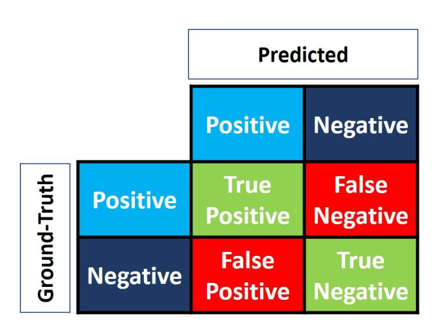
\includegraphics[width=0.8\linewidth]{pictures/Konfusionsmatrix_hs_analysis.png}
    \caption{Darstellung einer Konfusionsmatrix anhand von Annotationen (Ground-Truth) und Vorhersagen (Predicted) gemäß eines XNOR-Gatters}
    \label{fig:Konfusionsmatrix}
    \cite{noauthor_crc-modell_nodate}
\end{figure}

Precision
\begin{equation}
    Precision = \frac{\mbox{\textit{correctly classified actual positives}}}{\mbox{\textit{everything classified as positive}}} = \frac{TP}{TP + FP}
\end{equation}

Die Präzision beträgt im Idealfall ebenfalls 1,0 und hängt von der Anzahl falsch positiver Ergebnisse ab. Je geringer diese ist, desto besser die Genauigkeit. Präzision und Recall stehen sich in der Form gegenüber, als dass sie ein umgekehrtes Verhältnis haben und in der Regel mit steigender Präzision der Recall abnimmt und umgekehrt.

\begin{equation}
    Recall (\mbox{\textit{True Positive Rate, TPR}}) = \frac{\mbox{\textit{correctly classified actual positives}}}{\mbox{\textit{all actual positives}}} = \frac{TP}{TP + FN}
\end{equation}

Der Recall ist ein Indikator für die Erkennungswahrscheinlichkeit eines Modells, wobei ebenfalls ein Wert von 1,0 = 100\% angestrebt wird. Für die Anwendung an realen Datensätzen mit geringem Aufkommen positiver Ergebnisse bietet diese Berechnung mehr Aussagekraft als die Genauigkeit. Erfasst wird die Fähigkeit eines Modells zur richtigen Identifikation von positiven Instanzen.

\begin{equation}
    \mbox{\textit{FPR (False Positive Rate)}} = \frac{\mbox{\textit{incorrectly classified actual negatives}}}{\mbox{\textit{all actual negatives}}} = \frac{FP}{FP + TN}
\end{equation}

Die Wahrscheinlichkeit eines Fehlalarms, wie die Falsch-Positiv-Rate auch genannt wird, soll im Idealfall bei 0,0 und somit 0 \% liegen. Im Realfall ergibt sich die Aussagekraft aus der Anzahl von tatsächlichen Negativwerten und damit eine entsprechende Instabilität.

F1-Score
\begin{equation}
    2 * \frac{Precision * Recall}{Precision + Recall}
\end{equation}

Der F1-Score liefert den harmonischen Mittelwert anstelle des arithmetischen aufgrund der stärkeren Gewichtung von großen Unterschieden. Mit niedriger Precision oder Recall sinkt das Ergebnis selbst bei einem hohen Gegenwert, was ein schwerer zu manipulierendes Resultat bedeutet.

Accuracy
\begin{equation}
    Accuracy = \frac{\mbox{\textit{correct classifications}}}{\mbox{\textit{total classifications}}} = \frac{TP + TN}{TP + TN + FP + FN}
\end{equation}

Die Genauigkeit beschreibt den Anteil aller korrekten Klassifizierungen unabhängig von wahr oder falsch. Dies kann bei einer ausgewogenen Verteilung von TP und TN als eine ungefähre Übersicht für die Modellqualität dienen. Im Realfall liegen jedoch häufig unausgewogene Datensätze vor, bei denen entweder FN oder FP als Fehler überwiegt und damit die Aussagekraft reduziert. Entsprechend würde bei einem seltenen Aufkommen einer Klasse von nur 1\% das Modell in 100\% der Fälle \say{negativ} vorhersagen können, was in 99\% korrekt und dennoch nutzlos wäre.

Die Kürzel stehen für folgendes: TP = True Positive (wahre Positive), TN = True Negative (wahre Negative), FP = False Positive (falsche Positive) und FN = False Negative (falsche Negative).

Intersection over Union
\begin{equation}
    IoU = \frac{|A\cap B|}{|A\cup B|}
\end{equation}
Die Intersection over Union (zu Deutsch: Verhältnis der Schnittmenge zur Vereinigungsmenge, auch genannt Jaccard-Koeffizient) stellt ein Ähnlichkeitsmaß für Vektoren, Mengen und andere Objekte dar. Das dient der Beurteilung der Genauigkeit von Objekterkennungsmodellen und ihrer Optimierung. \cite{goodfellow_2016}

In der Form des Projekts stellt \textbf{IoU} die Schnittmenge der Ground-Truth-Pixelannotation und Vorhersage geteilt durch die Vereinigungsmenge derselben dar. Je ähnlicher Schnitt- und Vereinigungsmenge sind, desto mehr nähert sich der Wert eins an; bei vollständiger Übereinstimmung liegt er bei eins, bei keinerlei Übereinstimmung bei null. Die \textbf{mIoU} (\textbf{mean Intersection over Union}) beschreibt den durchschnittlichen IoU über mehrere Objekterkennungen zur besseren Gesamtakkuranz eines Modells. Da die Segmentierung pixelweise geschieht, ist der allgemeine Durchschnitt das geeignete Maß, solange das einzelne Objekt selbst keine Rolle spielt.

\textbf{Quantisierung/Optimierung für Edge-Geräte:} Um den Anspruch an die Rechenressourcen zu reduzieren, wird \textbf{Post Training Quantization (PTQ)} eingesetzt. Dabei wird die herkömmliche FP16-Aktivierungsausbreitung auf INT8 komprimiert, um den Speicherbedarf und die Inferenzlatenz auf dem Edge-Gerät zu senken. \textbf{Ergänzen}: Genauigkeitsverlust durch die Quantisierung anhand der obigen Metriken quantifizieren (FP16- vs. INT8-Modell). \cite{tensorflowPosttrainingQuantization}


%%%%%%%%%%%%%%%%%%%%%%%%%%%%%%%%%%%%%%%%%%%%%
%%%%%%%%%%%%%%%%%%%%%%%%%%%%%%%%%%%%%%%%%%%%%
%%%%%%%%%%%%%%%%%%%%%%%%%%%%%%%%%%%%%%%%%%%%%

%% Abkürzungsverzeichnis
% 	Befehl: makeindex Thesis.nlo -s nomencl.ist -o Thesis.nls
%
\input{references/acronyms.tex}

\markboth{\nomname}{\nomname}
\printnomenclature

%% Abbildungsverzeichnis
\listoffigures 

%% Tabellenverzeichnis
\listoftables 

%% Quelltextverzeichnis
\lstlistoflistings 

%% Stichwortverzeichnis
%	Befehl: makeindex Thesis
%
\printindex %\clearpage

%% Literaturverzeichnis
%	Befehl: biber Thesis

\printbibliography[heading=bibintoc, title={\babel{Literaturverzeichnis}{Bibliography}}]
%\clearpage
%Literaturverzeichnisse getrennt nach Stichwort
%\printbibliography[heading=bibintoc, keyword={book}, title={Literaturverzeichnis}]\clearpage
%\printbibliography[heading=bibintoc, keyword={online}, title={Onlinequellen}]\clearpage
%\printbibliography[heading=bibintoc, keyword={image}, title={Bildquellen}]\clearpage

%% Erklärung zur Eigenständigkeit
\input{Eigenstaendigkeitserklaerung}



\end{document}